\documentclass[11pt]{article}
\usepackage[T1]{fontenc}
\usepackage{lmodern}
\usepackage[margin=1in]{geometry}
\usepackage{amsmath,amssymb,amsthm,mathtools,mathrsfs,bm}
\usepackage{graphicx,tikz,enumitem,booktabs,microtype,etoolbox}
\usetikzlibrary{arrows.meta,positioning,calc,decorations.pathreplacing}
\usepackage[colorlinks=true,linkcolor=blue!45!black,citecolor=green!35!black,urlcolor=blue!55!black,bookmarksdepth=2,pdfauthor={OpenAI},pdftitle={Virasoro Constraints for Projective Complete Intersections}]{hyperref}
\usepackage[nameinlink,noabbrev]{cleveref}
\AddToHook{cmd/thebibliography/after}{\addcontentsline{toc}{section}{\refname}}
\makeatletter
\def\VirasoroThmRefstepcounter{%
  \@ifnextchar[{\VirasoroThmRefstepcounterOpt}%
    {\Hy@theorem@refstepcounter}}
\def\VirasoroThmRefstepcounterOpt[#1]#2{%
  \let\VirasoroSavedRefstepcounter\cref@old@refstepcounter
  \let\cref@old@refstepcounter\Hy@theorem@refstepcounter
  \refstepcounter@optarg[#1]{#2}%
  \let\cref@old@refstepcounter\VirasoroSavedRefstepcounter}
\patchcmd{\cref@thmnoarg}
  {\refstepcounter}{\VirasoroThmRefstepcounter}
  {}{\PackageError{virasoro}{Theorem anchor patch failed}{}}
\patchcmd{\cref@thmoptarg}
  {\refstepcounter}{\VirasoroThmRefstepcounter}
  {}{\PackageError{virasoro}{Typed theorem anchor patch failed}{}}
\makeatother
\theoremstyle{plain}
\newtheorem{theorem}{Theorem}[section]
\newtheorem{proposition}[theorem]{Proposition}
\newtheorem{lemma}[theorem]{Lemma}
\newtheorem{corollary}[theorem]{Corollary}
\theoremstyle{definition}
\newtheorem{definition}[theorem]{Definition}
\newtheorem{notation}[theorem]{Notation}
\newtheorem{example}[theorem]{Example}
\theoremstyle{remark}
\newtheorem{remark}[theorem]{Remark}
\crefname{theorem}{Theorem}{Theorems}
\crefname{proposition}{Proposition}{Propositions}
\crefname{lemma}{Lemma}{Lemmas}
\crefname{corollary}{Corollary}{Corollaries}
\crefname{definition}{Definition}{Definitions}
\crefname{notation}{Notation}{Notations}
\crefname{remark}{Remark}{Remarks}
\crefname{example}{Example}{Examples}
\crefname{section}{Section}{Sections}
\crefname{figure}{Figure}{Figures}
\newcommand{\C}{\mathbb C}
\newcommand{\Q}{\mathbb Q}
\newcommand{\R}{\mathbb R}
\newcommand{\Z}{\mathbb Z}
\newcommand{\PP}{\mathbb P}
\newcommand{\A}{\mathbb A}
\newcommand{\GW}{\mathrm{GW}}
\newcommand{\vir}{\mathrm{vir}}
\newcommand{\id}{\mathrm{id}}
\DeclareMathOperator{\Tr}{Tr}
\DeclareMathOperator{\str}{str}
\DeclareMathOperator{\ch}{ch}
\DeclareMathOperator{\codim}{codim}
\DeclareMathOperator{\rk}{rk}
\DeclareMathOperator{\coker}{coker}
\DeclareMathOperator{\im}{im}
\DeclareMathOperator{\Sym}{Sym}
\DeclareMathOperator{\End}{End}
\DeclareMathOperator{\Hom}{Hom}
\DeclareMathOperator{\Bl}{Bl}
\DeclareMathOperator{\ev}{ev}
\DeclareMathOperator{\pr}{pr}
\newcommand{\pt}{\mathrm{pt}}
\newcommand{\ot}{\otimes}
\newcommand{\h}{\hbar}
\newcommand{\HH}{H^*}
\newcommand{\cO}{\mathcal O}
\newcommand{\cM}{\mathcal M}
\newcommand{\cY}{\mathcal Y}
\newcommand{\cX}{\mathcal X}
\newcommand{\cD}{\mathcal D}
\newcommand{\cK}{\mathcal K}
\newcommand{\cA}{\mathcal A}
\pdfinfoomitdate=1
\pdfsuppressptexinfo=15
\pdftrailerid{}
\numberwithin{equation}{section}
\setlist{itemsep=3pt,topsep=5pt}
\setcounter{tocdepth}{1}
\title{Virasoro Constraints for Projective Complete Intersections}
\author{OpenAI}
\date{September 24, 2026}
\begin{document}
\maketitle
\begin{abstract}
We prove the Virasoro conjecture for the ordinary descendant
Gromov--Witten theory of smooth complete intersections in projective space,
in every genus and curve class and with arbitrary cohomology insertions.
This includes primitive and odd cohomology classes, with no semisimplicity
assumption.
\end{abstract}
\tableofcontents
\clearpage
\section{Introduction}\label{sec:introduction}

The Virasoro conjecture organizes the descendant Gromov--Witten invariants of a smooth projective variety into a system of differential equations. Its simplest instance is the intersection theory of the moduli spaces of curves: Witten's conjecture and Kontsevich's theorem identify the corresponding generating function with the distinguished solution of the KdV hierarchy \cite{Witten1991,Kontsevich1992}. Eguchi, Hori, and Xiong proposed a target-dependent Virasoro system for Fano varieties \cite{EHX1997}. Eguchi, Jinzenji, and Xiong extended the free-field formulation to odd and off-diagonal Hodge classes, crediting Katz's proposal to use a Hodge index in the grading \cite{EJX1998}. We use the first-Hodge-degree superspace operators and central normalization of Getzler \cite{Getzler1999}.

For a smooth projective variety $X$, let $F_g^X(t)$ be the generating series of its ordinary, unreduced genus-$g$ descendant invariants. The variables $t_m^a$ record insertions $\tau_m(\phi_a)$ for a homogeneous cohomology basis $\{\phi_a\}$, and Novikov variables record curve classes. The total descendant potential is
\[
 Z_X(t)=\exp\!\left(\sum_{g\geq0}\h^{g-1}F_g^X(t)\right).
\]
The conjecture asserts
\[
 L_k^X Z_X=0\qquad(k\geq-1),
\]
where the target-dependent differential operators $L_k^X$ are formed from the Poincar\'e pairing, the first Hodge index $p$ on $H^{p,q}(X)$, and cup product with $c_1(TX)$. Their precise quantization, super signs, and scalar normalization are fixed in \cref{sec:conventions}. All equations are formal coefficientwise identities.

\begin{theorem}\label{thm:main}
Let \(X\subset\PP^N_\C\) be a smooth complete intersection. Its ordinary, unreduced total descendant potential satisfies the Virasoro constraints in every genus and curve class, with arbitrary insertions from \(H^*(X;\C)\).
\end{theorem}

Thus \cref{thm:main} resolves the Virasoro conjecture positively for projective-space complete intersections. Primitive and odd insertions are included, with no semisimplicity hypothesis.

The genus-zero constraints are known in general. Liu and Tian proved the decisive $L_1$ and $L_2$ identities for even-class inputs without a Fano hypothesis \cite[Theorem~0.2]{LiuTian1998}. Dubrovin and Zhang proved the genus-zero Frobenius-manifold formulation and the semisimple genus-one case \cite[Main Theorem]{DubrovinZhang1999}; Getzler treated the genus-zero superspace formulation used here \cite[Section~4]{Getzler1999}.

Several all-genus cases are also established. Getzler proved the ordinary constraints for Calabi--Yau targets with $c_1(X)=0$ and $H^1(X)=0$ \cite[Theorem~7.1]{Getzler1999}. Okounkov and Pandharipande proved the fixed-degree relative constraints for target curves, including odd descendants \cite[Theorem~3]{OP2003}. Givental's quantized semisimple construction, together with Teleman's classification, covers the corresponding homogeneous semisimple geometric theories \cite{Givental2001,Teleman2012}. More recently, Guo, Zhang, and Zhou proved genus-one constraints on the ambient state space of smooth Fano complete intersections and announced further full-cohomology genus-one extensions for several families, with details deferred to a forthcoming paper \cite[Theorem~1 and Remark~3.10]{GuoZhangZhou2026}. The present argument addresses all genera and all insertions simultaneously through degeneration.

\subsection{Degeneration and primitive cohomology}

Degeneration expresses Gromov--Witten invariants through relative invariants of simpler pieces \cite{Li2001,Li2002,AF2016}. Relative reconstruction and equation splitting were developed by Maulik and Pandharipande \cite{MaulikPandharipande2006}. Arg\"uz, Bousseau, Pandharipande, and Zvonkine used nodal invariants to reconstruct the full Gromov--Witten theory of complete intersections by induction on dimension and defining degrees \cite[Theorem~5.3 and Section~5.3]{ABPZ}. We use the same geometric reduction; the additional objective is to transport the Virasoro equations, including their first-Hodge-weighted contractions.

The reduction has two stages. Factoring one defining equation and resolving the resulting family gives a degeneration
\[
 X\rightsquigarrow U\cup_D\widetilde M,
 \qquad \widetilde M=\Bl_S M.
\]
Here $U$ and $M$ are complete intersections of smaller defining degree, while the seam $D$ and blowup center $S$ have smaller dimension. We first prove the constraints for $\widetilde M$ from those for $M$ and projective-bundle towers over $S$. We then prove them for $X$ from those for $U$, $\widetilde M$, and a ruled bundle over $D$. The needed bundles are towers of projectivizations of sums of line bundles, so toric-bundle transfer supplies their constraints from those of their bases \cite{CGT}. \Cref{ind:section} carries out this induction and verifies the first-Hodge convention in the bundle transfer.

Two difficulties prevent an immediate deduction from the numerical degeneration formula. Primitive insertions need not extend individually through a degeneration. Moreover, the Virasoro operators weight contracted indices by their first Hodge degrees, so their contractions cannot be treated as ungraded diagonal insertions. For fixed genus, degree, and descendant orders, we regard the coefficient of $L_k^X Z_X$ as a multilinear error tensor in its cohomology inputs. We transport scalar contractions of this tensor with coherently extending classes of fixed Hodge type, graded inverse pairings, and ordinary Gromov--Witten tensors from independent copies of the theory. These are the tests that will detect the error without extending each primitive input.

\subsection{The transport argument}

The transport needed in both stages rests on three constructions.

First, contractions are performed on the first page of the weight spectral sequence. Its pairing is perfect at the level of complexes and has an inverse tensor supported at vertices and edges of the degeneration graph. The first Hodge degree, including Tate twists, commutes with its differential. Multiplicative comparison and trace then evaluate the contracted tensor without choosing representatives in the surviving cohomology. We use Steenbrink's limiting mixed Hodge structures and Fujisawa's ordered model, multiplicative comparison, and trace \cite{Steenbrink1976,Steenbrink1977,Fujisawa2008,Fujisawa2014}.

For this calculation, the virtual class pushed forward by evaluation at the recorded markings must extend to a resolved product of the family. Configurations of points on common expansions provide that product \cite{AFConfigurations}. We compute its component restrictions by virtual splitting before integration, keeping the recorded markings' component assignments. When disconnected groups of maps are separated, we retain the joint evaluation of the group carrying those markings. These correspondence statements are stronger than a numerical degeneration identity and are proved in \cref{ev:section}.

Second, relative caps reproduce the contact pairing at a seam. Ordinary descendants on one cap realize functionals on a bounded incoming contact space; descendants on the other prepare the corresponding states with all unwanted outgoing profiles canceled. The nonzero projective-space fiber invariants of Hu, Li, and Ruan \cite{HLR2008} give the invertible linearization from which the full disconnected cap construction begins. In the blowup configuration, corrections of counting degree zero strictly decrease contact. Together with degree bounds, this makes every required inversion coefficientwise finite.

Insert many widely separated switches into a degeneration with a long chain of ruled components. At a switch, either keep the original joining or separate the two sides and add the prepared caps. The cap tests may use many auxiliary markings, but their ordinary insertions are integrated into the evaluation correspondence. A quadratic Virasoro operator modifies at most two existing labels. Thus the exposed cohomological operations occupy a bounded number of positions, independently of the auxiliary markings. The alternating sum over switch choices cancels by toggling the first switch away from these positions; see \cref{fig:sewing}. Every nonempty surgery subset smooths to a disjoint union of the shorter targets described above, whose absolute constraints are known. The cancellation therefore proves every such scalar test of the error on the original target.

Third, these tests detect all primitive tensors. Hodge--Riemann gives a positive Hermitian form on primitive middle cohomology. Pairing a Virasoro error tensor with its conjugate in a second replica produces its squared norm. The contraction is among the allowed tests, and positivity forces the tensor itself to vanish. This argument has no bound on the number of primitive insertions.

Transport initially gives coefficients selected by the divisor degrees that extend coherently through the degenerations. To obtain the asserted result in each curve class, we verify that these degrees separate all relevant classes, retaining additional divisor degrees for exceptional surfaces and blowups. Deformation invariance and the same scalar-test argument then give the constraints on every smooth member. These are part of the final induction, not extra hypotheses on \cref{thm:main}.

\begin{figure}[ht]
\centering
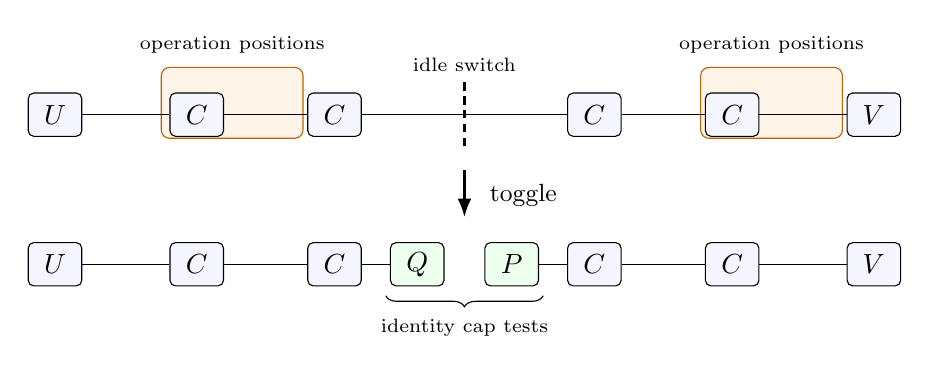
\begin{tikzpicture}[x=1cm,y=1cm,>=Latex,
  piece/.style={draw,rounded corners=2pt,minimum width=.68cm,minimum height=.55cm,fill=blue!4},
  cappiece/.style={draw,rounded corners=2pt,minimum width=.68cm,minimum height=.55cm,fill=green!7},
  busy/.style={draw=orange!75!black,fill=orange!9,rounded corners=3pt}]
\filldraw[busy] (1.35,.35) rectangle (3.15,1.25);
\filldraw[busy] (8.2,.35) rectangle (10,1.25);
\node[font=\scriptsize,anchor=south] at (2.25,1.30) {operation positions};
\node[font=\scriptsize,anchor=south] at (9.1,1.30) {operation positions};
\foreach \i/\x/\s in {0/0/U,1/1.8/C,2/3.55/C,3/6.85/C,4/8.6/C,5/10.4/V}
  {\node[piece] (t\i) at (\x,.65) {\(\s\)};}
\draw (t0)--(t1);
\draw (t1)--(t2);
\draw (t2)--(t3);
\draw (t3)--(t4);
\draw (t4)--(t5);
\draw[densely dashed,thick] (5.2,.25)--(5.2,1.07);
\node[font=\scriptsize,above] at (5.2,1.07) {idle switch};
\draw[->,thick] (5.2,-.05)--(5.2,-.65);
\node[font=\small,right] at (5.4,-.37) {toggle};
\foreach \i/\x/\s in {0/0/U,1/1.8/C,2/3.55/C,3/6.85/C,4/8.6/C,5/10.4/V}
  {\node[piece] (b\i) at (\x,-1.25) {\(\s\)};}
\node[cappiece] (Q) at (4.6,-1.25) {\(Q\)};
\node[cappiece] (P) at (5.8,-1.25) {\(P\)};
\draw (b0)--(b1);
\draw (b1)--(b2);
\draw (b2)--(Q);
\draw (P)--(b3);
\draw (b3)--(b4);
\draw (b4)--(b5);
\draw[decorate,decoration={brace,mirror,amplitude=4pt}] (4.2,-1.65)--(6.2,-1.65);
\node[font=\scriptsize,below] at (5.2,-1.82) {identity cap tests};
\end{tikzpicture}
\par

\caption{One idle switch in the transport argument. Here \(U,V\) are the ends, \(C\) is a ruled neck, and \(P,Q\) are replacement caps; see \cref{sew:configurations}. The marked neighborhoods carry the fixed cohomological operations. At a switch outside those neighborhoods, the prepared combination of cap tests reproduces the original contact identity. Toggling that switch changes the inclusion--exclusion sign and preserves the retained tensor data.}
\label{fig:sewing}
\end{figure}

\subsection{Organization and scope of the inputs}

\Cref{sec:conventions} specifies the operators, tensor tests, and completions. \Cref{fp:section,ev:section} establish the local Hodge calculation and its evaluation correspondence. \Cref{cap:section} constructs the cap tests, and \cref{sew:section} proves their transport theorem. \Cref{sec:detection} gives the positivity detector. \Cref{ind:section} assembles these results in the complete-intersection induction, including the surface and curve-class arguments.

Established degeneration, limiting-Hodge, toric-bundle, and intersection-theoretic results are used with their stated hypotheses. The local correspondence calculation, bounded cap preparation, grouped switch cancellation, and primitive tensor detector are proved here. In particular, the sewing theorem is not attributed to the numerical degeneration formula. The toric-bundle step explicitly passes from a half-total-degree convention to first Hodge degree at Hodge-neutral auxiliary parameters, with the corresponding central normalization.

\section{Operators, tensor tests, and conventions}\label{sec:conventions}

\subsection{The descendant theory}

All varieties are smooth and projective over \(\C\), unless they occur as fibers of a specified semistable family. Cohomology has complex coefficients and its usual parity. Tensor products, symmetric powers, permutations, and derivatives are taken in super vector spaces. For a target \(X\) of complex dimension \(n\), write
\[
 (a,b)_X=\int_X a\cup b,\qquad
 \mu_X|_{H^{p,q}(X)}=(p-n/2)\id,\qquad
 \mathcal R_X(a)=c_1(TX)\cup a.
\]
The pairing is perfect and even. Its coevaluation is the categorical inverse of this pairing; it includes the signs dictated by the super symmetry. We never insert a second parity involution into a node kernel.

Choose a Hodge-homogeneous basis \(\{\phi_a\}\) and let
\(t(z)=\sum_{m\geq0,a}t_m^a\phi_a z^m\), where \(t_m^a\) has the parity of \(\phi_a\). The connected potentials and total descendant potential are
\begin{align}
 F_g^X(t)
 &=\sum_{\beta}\sum_{r\geq0}
   \frac{\mathsf Q^\beta}{r!}
   \int_{[\overline{\cM}_{g,r}(X,\beta)]^\vir}
        \prod_{i=1}^r\left(\sum_{m,a}t_m^a\psi_i^m\ev_i^*\phi_a\right),
 \label{eq:potential}\\
 Z_X(t)&=\exp\left(\sum_{g\geq0}\h^{g-1}F_g^X(t)\right).
 \label{eq:partition}
\end{align}
Only stable maps contribute. The \(\psi_i\) are cotangent classes at markings on the source of the stable map, not classes pulled back by stabilization to curves. In particular, the same convention is used in relative theories and in the fiber calculation below.

Equation \eqref{eq:partition} packages disconnected domains, with the empty domain contributing \(1\). We use labelled coefficient extraction to discuss multilinear tensors: distinct formal variables distinguish all prescribed insertions, even when their values coincide. This convention accounts automatically for the factorials in \eqref{eq:potential}.

All statements are coefficientwise. Fixing an ample integral curve degree, a finite list of markings, and a genus coefficient leaves finite sums of effective curve classes and discrete stable-map data. In intermediate relative theories we impose the additional contact and end-degree bounds specified in the cap construction. Laurent series in \(\h\) are always bounded below at the finite auxiliary-variable and degree orders in use. For several replicas, the genus and curve variables are independent. The cap construction proves the corresponding boundedness when the counting polarization is only relatively ample.

\subsection{The positive Virasoro operators}

Let
\[
 \mathcal H_X=H^*(X)((z^{-1})),\qquad
 \Omega_X(f,g)=\operatorname*{Res}_{z=0}(f(-z),g(z))_X\,dz.
\]
With the standard polarization
\(\mathcal H_X=H^*(X)[z]\oplus z^{-1}H^*(X)[[z^{-1}]]\), set
\begin{equation}
 \ell_0=z\partial_z+\tfrac12+\mu_X+\frac{\mathcal R_X}{z},
 \qquad
 \ell_k=\ell_0(z\ell_0)^k\quad(k\geq1).
 \label{eq:loop-operators}
\end{equation}
These are infinitesimal symplectic operators. For example,
\(\mu_X^*=-\mu_X\), \(\mathcal R_X^*=\mathcal R_X\), and the sign from \(z\mapsto-z\) gives the required adjoints. The quadratic Hamiltonian of \(\ell_k\) is quantized with normal ordering. In Darboux coordinates this sends terms \(pp,pq,qq\), respectively, to \(\h\) times second derivatives, first-order vector fields, and multiplication by a quadratic polynomial divided by \(\h\). Apply the dilaton translation
\[
 q(z)=t(z)-z\,1_X.
\]
Up to the harmless simultaneous operator-sign convention, these are the positive operators \(L_k^X\) in Getzler's formulation \cite[Equation~(1.2)]{Getzler1999}. There is no central scalar correction for \(k>0\). We fix the signs by that reference when invoking the Virasoro commutators.

For clarity, the proof uses the following finite description rather than a coordinate expansion of every coefficient.

\begin{proposition}[Positive coefficient rule]\label{conv:positive-rule}
A labelled coefficient of \(L_k^XZ_X\), for fixed \(k>0\), is a finite linear combination of the following operations on the disconnected Gromov--Witten tensors:
\begin{enumerate}[label=\textup{(\roman*)}]
\item add one special unit marking, with prescribed descendant and \(\mathcal R_X\)-powers;
\item act on one existing marking, changing its descendant exponent and applying an \(\mathcal R_X\)-power, with a coefficient polynomial in its first Hodge degree;
\item add two markings joined by the coevaluation of \((\, ,\,)_X\), with descendant powers, first-Hodge-degree polynomials, and \(\mathcal R_X\)-powers on its legs;
\item remove two primary markings, leaving their two cohomology inputs in the classical pairing with \(\mathcal R_X^{k+1}\), multiplied by the remaining disconnected Gromov--Witten tensor.
\end{enumerate}
The numerical coefficients and genus powers are universal for targets of fixed dimension. At most two existing labels are used nonordinarily in one summand.
\end{proposition}

\begin{proof}
Expand \(\ell_0(z\ell_0)^k\) using
\([z\partial_z,z]=z\) and \([\mu_X,\mathcal R_X]=\mathcal R_X\).
The resulting coefficients are polynomials in the first Hodge index, composed with Chern-class powers. The three blocks of its quadratic Hamiltonian give the last three types of operation under normal ordering; the dilaton shift gives the special unit marking. The block with both variables on the positive polarization has its only relevant negative shift at the primary pair, giving the classical \(\mathcal R_X^{k+1}\)-pairing. This is also the three-block decomposition in the cited coordinate formula. Since the Hamiltonian is quadratic, at most two existing labels are involved. Super quantization uses the same calculation with graded derivatives and permutations.
\end{proof}

The two lower operators are the standard string operator \(L_{-1}\) and the quantization of \(\ell_0\) with scalar
\[
 C_X=\frac{\chi(X)}{16}-\frac14\str(\mu_X^2),
\]
in Getzler's first-Hodge convention; its Chern-number form appears in \eqref{ind:central-normalization}. The nonpositive constraints require no new transport theorem. The string equation gives \(L_{-1}Z_X=0\). Together with \(L_1Z_X=0\), the commutator \([L_1,L_{-1}]=2L_0\) gives \(L_0Z_X=0\) with this normalization. Equivalently one may use the usual dilaton, homogeneity, divisor, and genus-one Riemann--Roch identities. We therefore prove all positive constraints.

\subsection{Admissible scalar tests}

An \emph{ordinary replica} means a separate copy of a disconnected Gromov--Witten tensor, with its own genus and degree variables. A \emph{tested positive constraint} consists of one coefficient rule from \cref{conv:positive-rule}, applied to one specified replica, followed by a finite tensor contraction using:
\begin{enumerate}[label=\textup{(\alph*)}]
\item ordinary replicas and classical cup integrals;
\item single classes obtained from algebraic classes on the relevant total families, allowing complex linear combinations and including units and Chern-class powers, or from homogeneous cohomology classes of fixed smooth projective sources through algebraic correspondences extending over those total families and inducing flat Hodge maps on their smooth loci;
\item coevaluations joining arbitrary pairs of slots, possibly on different replicas;
\item polynomials, or functions on the finite spectrum, of the first Hodge degree on any exposed leg;
\item cups with admissible single classes and numerical coefficients.
\end{enumerate}
The arities of this test are fixed. Only the chosen replica is acted on by \(L_k\); the test is then applied linearly to its coefficients. The test may be different for each coefficient that is to be proved zero.

When auxiliary cap markings are later inserted in the chosen replica, \(L_k\) acts on those variables as well. Their ordinary occurrences are preintegrated into the evaluation correspondence. If the coefficient rule modifies one of them, or removes it into a classical pairing, it is exposed as an additional position. By \cref{conv:positive-rule}, there are at most two such positions. Auxiliary cap labels on other replicas remain ordinary.

All contractions can be decomposed into homogeneous Hodge types. For a single supplied by a fixed smooth projective source, keep its cohomology slot exposed until the extending algebraic correspondence has been specialized; the homogeneous input itself need not be algebraic. A topologically extending class alone is not sufficient: its Hodge components need not be flat. Nor do we assert tested transport for an arbitrary flat Hodge correspondence without the specified algebraic extension over the total family. The first-index operations are permitted only in balanced numerical diagrams: the types of the algebraic correspondences, cups, and pairings must match the total input and output types. The limiting-Hodge calculation below explains why these numerical contractions are constant in smooth families and admit the required graded specialization.

\begin{definition}[Coherent data]\label{conv:coherent}
Admissible singles and numerical divisor-degree tests on several degenerations are \emph{coherent} if their restrictions agree on the common local component and stratum diagrams used in the comparison. For source-supplied singles this agreement is required for the specified extending algebraic correspondences with their cohomology slots exposed, before applying the fixed inputs. A class supported at a specified unaffected end is taken to have zero restriction on the other ends and replacement caps.
\end{definition}

The Chern-class insertion always has a coherent choice. The extension
\(-c_1(\omega_{\cY/B})\) restricts on a component \(Y_i\) with boundary \(D_i\) to \(c_1(TY_i)-[D_i]\), the logarithmic first Chern class. The local calculations use this class. They do not replace it silently by \(c_1(TY_i)\).

The tensor manipulations do not require individual primitive insertions to extend. They use full coevaluations and finitely many coherent singles; the final detection argument recovers arbitrary primitive inputs only on the target being proved.

\section{First-page contractions and locality}\label{fp:section}

The inverse Poincar\'e pairing on a nearby fiber need not have a useful
expression in terms of surviving classes on the components of a degeneration.
We instead use an inverse pairing on a complex.  Its individual terms have
small support, although only their sum is closed.  The distinction is essential:
we identify a numerical contraction using the closed sum, and subsequently
expand that sum into local terms.

Throughout this section, $\pi:\cY\to\Delta$ is a projective semistable family
of relative dimension $n$, with smooth total space.  Its central fiber
$Y=\bigcup_{v\in V}Y_v$ has smooth components and no triple intersections.
Its dual graph is bipartite.  We orient each edge from color $0$ to color $1$.
An edge $e$ denotes a connected component $D_e$ of a double locus; its two
inclusions are $i_{e,0}$ and $i_{e,1}$.  Disconnected total spaces are allowed.
All cohomology is rational unless complex coefficients or Hodge decompositions
are specified.  The Tate structure $\Q(-1)$ has Hodge type $(1,1)$.
The parity in a complex is its \emph{total} cohomological degree.

\subsection{The three-column complex}

We use the weight spectral sequence with indexing
\begin{equation}\label{fp:eone}
 E_1^{-1,b}=\bigoplus_e H^{b-2}(D_e)(-1),\qquad
 E_1^{0,b}=\bigoplus_v H^b(Y_v),\qquad
 E_1^{1,b}=\bigoplus_e H^b(D_e).
\end{equation}
All other columns are zero.  The differential $d_1$ increases the first index
by one and preserves the second.  Write $C_Y=\operatorname{Tot}(E_1,d_1)$.
There are identifications
\begin{equation}\label{fp:total-complex}
 C_Y^k=\bigoplus_v H^k(Y_v)
 \oplus\bigoplus_e H^{k-1}(D_e)
 \oplus\bigoplus_e H^{k-1}(D_e)(-1).
\end{equation}
Denote the last two kinds of elements by $a$ and $b$, respectively.  We choose
the signs of the residue identifications so that
\begin{equation}\label{fp:differential}
 d(v,a,b)=(\gamma b,\rho v,0),\qquad
 (\rho v)_e=i_{e,1}^*v_1-i_{e,0}^*v_0,
 \qquad
 \gamma b=\sum_e\bigl(-i_{e,0*}b_e+i_{e,1*}b_e\bigr).
\end{equation}
Here a term of $\gamma$ belongs to the indicated component summand.
These conventions are isomorphic to the usual residue conventions by signs
on the summands.

For completeness, $\rho\gamma=0$ can be seen directly.  Distinct double loci
on a fixed component are disjoint.  At $D_e$, the remaining composition is
multiplication by
$c_1(N_{D_e/Y_0})+c_1(N_{D_e/Y_1})$, which is zero because the two normal
bundles are dual in a semistable smoothing.  Thus \eqref{fp:differential}
is a differential.

The Steenbrink theorem identifies
\begin{equation}\label{fp:abutment}
 H^k(C_Y)=\bigoplus_a E_2^{a,k-a}
 =\bigoplus_a\operatorname{Gr}^{W}_{k-a}H^k(Y_t)_{\mathrm{lim}},
\end{equation}
with its pure Hodge structures and the displayed Tate twists; the weight
spectral sequence degenerates at $E_2$
\cite{Steenbrink1976,Steenbrink1977}.
Here $W$ on the right is the usual weight filtration of the limiting mixed
Hodge structure.  In filtered-complex notation below, this incorporates the
usual shift by cohomological degree.

\begin{lemma}[The first-page pairing]\label{fp:pairing}
The complex $C_Y$ has a perfect graded-symmetric chain pairing of degree $2n$
and Tate type $\Q(-n)$.  On elements of total degrees $k$ and $2n-k$ it is
\begin{align}\label{fp:pairing-formula}
 B_Y\bigl((v,a,b),(w,a',b')\bigr)
 ={}&\sum_v\int_{Y_v}v_v\cup w_v
       +(-1)^k\sum_e\int_{D_e}a_e\cup b'_e\\
    &+(-1)^{k+1}\sum_e\int_{D_e}b_e\cup a'_e.\notag
\end{align}
It induces the weight-graded nearby Poincar\'e pairing under
\eqref{fp:abutment}.  Its categorical inverse-pairing tensor $\Delta_{C_Y}$
is closed and is a sum of tensors supported on a single vertex or a single
edge.
\end{lemma}

\begin{proof}
Perfection follows from Poincar\'e duality on the smooth projective $Y_v$ and
$D_e$.  The edge summands pair with one another, not with themselves.  Ordinary
cup-commutativity gives graded symmetry with respect to total degree.
The projection formula says that $\gamma$ is transpose to $\rho$ before the
shift signs.  If $x$ is in a component summand of degree $k$ and $y$ is in a
$b$ summand of degree $2n-k-1$, the two terms of
\begin{equation}\label{fp:chain-pairing}
 B_Y(dx,y)+(-1)^k B_Y(x,dy)=0
\end{equation}
are $(-1)^{k+1}\int \rho x\cup y$ and
$(-1)^k\int \rho x\cup y$.  They cancel.  The case with the $b$ summand
first follows in the same way, and all other cases vanish.  This proves the
chain identity.

We specify the compatibility with nearby integration below, in
\cref{fp:trace-normalization}; it uses the multiplicative comparison and
trace of Fujisawa.  The residue calculation identifying that trace pairing
with \eqref{fp:pairing-formula} is
\cite[Lemma~6.13 and proof of Theorem~8.11]{Fujisawa2014}, after the sign
choices in \eqref{fp:differential}.  Thus this compatibility does not require
choosing representatives for the groups in \eqref{fp:abutment}.

A perfect chain pairing identifies a finite complex with its shifted dual.
Under this identification its inverse-pairing tensor corresponds to the
identity chain map.  It is therefore closed.  Finally,
\eqref{fp:pairing-formula} is block diagonal by vertices and by edges, so its
inverse has the asserted support.  All inverse tensors here and below use
the categorical Koszul convention.
\end{proof}

\begin{lemma}[First Hodge index]\label{fp:first-index}
On $C_Y\otimes\C$, let $P$ act by the first Hodge index, including the Tate
twist.  Then $Pd=dP$.  Consequently $(f(P)\otimes\id)\Delta_{C_Y}$ is closed
for every function $f$ on the finite spectrum of $P$.
\end{lemma}

\begin{proof}
A restriction preserves Hodge type.  A Gysin map raises both Hodge indices
by one, exactly as does the twist in its source $b$ summand.  Thus both arrows
of \eqref{fp:differential} preserve the first index.  The last assertion
follows by applying a chain map to a closed tensor.  Notice that the total
cohomological degree operator does not have this property: $d$ raises total
degree by one.
\end{proof}

\begin{example}\label{fp:curve-example}
Let two rational curves meet in $m$ nodes, where $m=1$ or $2$.  Choose component
units $u_0,u_1$, top classes $t_0,t_1$, and node generators $a_e,b_e$.
Then
\[
 du_0=-\sum_ea_e,\qquad du_1=\sum_ea_e,\qquad
 db_e=-t_0+t_1.
\]
The first Hodge indices of $u,a,b,t$ are $0,0,1,1$.  The inverse tensor is
\[
 \Delta_{C_Y}=\sum_{i=0}^1(u_i\otimes t_i+t_i\otimes u_i)
          +\sum_{e=1}^m(a_e\otimes b_e-b_e\otimes a_e).
\]
Its differential vanishes by cancellation between vertex and edge terms.
For $m=1$ the cohomology dimensions are $(1,0,1)$; for $m=2$ they are
$(1,2,1)$.  Thus the construction includes the graph contribution to nearby
$H^1$.  Individual vertex and edge terms are usually not closed.
\end{example}

\subsection{Filtered multiplicative models and ordered pullbacks}

We use the ordered polynomial-log model of
\cite[Sections~4.14--4.19 and~5.4, Proposition~5.8]{Fujisawa2008}.
In that model each nonempty subset of component indices occurs once, in its
increasing order.  This choice matters: it is not the unrestricted complex
of all injective ordered tuples.  Let $A_Z$ be the Steenbrink complex for a
projective semistable central fiber $Z$, now allowing higher intersections,
and write $K_Z$ for this ordered model.  The standard hypotheses are
properness and smooth K\"ahler components, which hold for our projective
models.  The comparison used below is a bifiltered map
\begin{equation}\label{fp:comparison}
 \phi_Z:A_Z\longrightarrow K_Z
\end{equation}
inducing the limiting mixed-Hodge isomorphism and an isomorphism on second
weight pages.  We give the ordered interpretation of this comparison and
of the trace explicitly, so no identification of different \v{C}ech
conventions is implicit.

Here is the structure of the model that will be used.  If $I$ is a nonempty
set of component indices, $Z_I$ is their intersection with the induced
absolute log structure and $\omega_{Z_I}$ its absolute log de Rham complex.
The local terms are
\[
 \C[u]\otimes\omega_{Z_I},\qquad
 \nabla=1\otimes d+(2\pi\sqrt{-1})^{-1}
                      \partial_u\otimes(d\log s\wedge).
\]
Their component \v{C}ech total complex is $K_Z$.  A power $u^r$ has weight
$2r$ and first Hodge degree $r$.  In \v{C}ech degree $j$ its filtrations are
\begin{align}\label{fp:k-filtrations}
 W_m K_Z&=\sum_{r\geq0}u^r\otimes W_{m+j-2r}\omega_{Z_I},&
 F^pK_Z&=\sum_{r\geq0}u^r\otimes F^{p-r}\omega_{Z_I}.
\end{align}
The $W$ on forms counts logarithmic factors.  Residues describe its graded
pieces by ordinary forms on closed intersections.  The map $\phi_Z$ is a sum
of residue maps multiplied by divided powers of $u$, with universal signs
and Tate factors.  Its summands only involve incident strata
\cite[Definition~5.24 and Lemma~5.25]{Fujisawa2014}.

Multiplication in $K_Z$ is polynomial multiplication, wedge product, and the
ordered \v{C}ech Alexander--Whitney product, with its total-complex signs.
The formulas in \cite[Sections~6.1--6.8]{Fujisawa2014} apply to increasing
tuples: the two overlapping subtuples of an increasing tuple are increasing.
Thus the product is a chain map preserving both filtrations.  Evaluation at
$u=0$ followed by passage to relative log forms respects this product, so its
cohomological product is ordinary nearby cup product.

\begin{lemma}[Ordered comparison]\label{fp:ordered-comparison}
The residue formula for $\phi_Z$, restricted to increasing tuples, gives
\eqref{fp:comparison} with the properties stated above.
\end{lemma}

\begin{proof}
Restriction of a cochain indexed by all injective ordered tuples to increasing
tuples commutes with the \v{C}ech differential, because every face of an
increasing tuple is increasing.  It commutes with the internal differential
and preserves \v{C}ech degree and the two filtrations.  Consequently restricting
the explicit residue map of \cite[Definition~5.24 and Lemma~5.25]{Fujisawa2014}
gives a bifiltered chain map into the ordered model.  This conclusion only
uses the formula and its chain identity, not a quasi-isomorphism assertion
for an unrestricted tuple complex.

Evaluate at $u=0$ and pass to relative log forms.  The comparison square in
\cite[proof of Theorem~5.29]{Fujisawa2014} remains commutative after this
restriction: its equality is an equality of residue maps on each intersection.
Its other arrows are the Steenbrink comparison with relative log de Rham
cohomology, the ordered relative-log \v{C}ech resolution
\cite[Proposition~4.19]{Fujisawa2008}, and the polynomial-log comparison
\cite[Lemma~5.6 and Corollary~5.7]{Fujisawa2008}.  All three induce
isomorphisms on cohomology.  Therefore so does $\phi_Z$.  The rational
comparison is obtained by the same restricted Koszul-residue formula, and
it has the same compatibility with Tate factors as the complex comparison.
The source is a cohomological mixed Hodge complex, and the ordered target
is a weak cohomological mixed Hodge complex by
\cite[Proposition~5.8]{Fujisawa2008}.  Its cohomology carries the mixed
Hodge structure of \cite[Theorem~5.9]{Fujisawa2008}, and its weight spectral
sequence degenerates at $E_2$ by \cite[Lemma~A.6]{Fujisawa2008}.
Thus the cohomological isomorphism is one of mixed Hodge structures.
Weight degeneration and strictness now give
the asserted isomorphism of second pages, exactly as in
\cite[Corollary~5.30]{Fujisawa2014}.
\end{proof}

Let $\widetilde{\cY^{\,r}}$ be the ordered semistable configuration model for
$r$ recorded points, as in \cref{ev:restriction}.  Locally it resolves
\[
 x_i y_i=s,\qquad 1\leq i\leq r,
\]
by the ordered triangulation of $[0,1]^r$.  Its vertices are assignments of
components to the recorded points, and its simplices are chains of assignments
in the coordinatewise order.  Color $0$ precedes color $1$ in each factor.
Order all vertices by the number of color-$1$ coordinates, breaking ties
arbitrarily.  This order is strictly increasing on every nonconstant step in
such a simplex.  Each coordinate projection is therefore weakly increasing
on each ordered simplex.  The same statement applies when some coordinates
are fixed off the double locus, and on disconnected pieces.  Only assignments
lying on a common simplex matter; there is no comparison of points on
disjoint strata.

\begin{lemma}[Ordered pullbacks]\label{fp:pullback}
Each projection of the ordered configuration model to $\cY$ induces a
bifiltered chain pullback of the $K$ models.  On weight pages its terms are
ordinary pullbacks on the relevant intersections and the maps on logarithmic
generators modulo ordinary forms.  These terms are determined by the incident
strata, their normal data, and the chosen ordering.
\end{lemma}

\begin{proof}
Write $f$ for the component assignment of a projection.  For a source
increasing tuple $J=(j_0,\ldots,j_k)$, the component of the pullback of a
\v{C}ech cochain $\eta$ is
\begin{equation}\label{fp:cech-pullback}
 (f^*\eta)_J=
 \begin{cases}
 f_J^*\eta_{f(j_0),\ldots,f(j_k)},&
                 f(j_0)<\cdots<f(j_k),\\
 0,&\text{some projected vertices repeat}.
 \end{cases}
\end{equation}
In the second case the tuple is degenerate.  Formula
\eqref{fp:cech-pullback} commutes with the \v{C}ech differential: if a projected
tuple has exactly one adjacent repetition, deleting either member produces
the same restriction with opposite signs; all other faces remain degenerate.
More repetitions give zero on both sides, and distinct tuples give the usual
pullback identity.  Weak monotonicity ensures that repetitions are adjacent.
This also makes \eqref{fp:cech-pullback} compatible with the
Alexander--Whitney product: a repeated adjacent pair lies in at least one of
the two overlapping subtuples used by that product.

On each intersection use the pullback of absolute log forms and set
$f^*u=u$.  The morphism is over the same base, so $f^*d\log s=d\log s$;
it commutes with $\nabla$.  Ordinary forms pull back to ordinary forms, while
a local log generator pulls back to a sum of log generators and an ordinary
form.  Thus log weight and form degree do not increase.  Every nonzero term
of \eqref{fp:cech-pullback} retains the same \v{C}ech degree, so
\eqref{fp:k-filtrations} proves preservation of both filtrations.

Finally, take residues.  Ordinary corrections to a logarithmic generator
have zero residue, and the remaining maps only use its orders along the
incident divisors.  A unit change of a local boundary equation does not change
these residue maps.  This proves the asserted dependence and locality.
\end{proof}

\subsection{Trace and specialization of correspondences}

If $Z$ has pure dimension $N$, the ordered model has a first-page functional
\begin{equation}\label{fp:theta}
 \Theta_Z:E_1^{0,2N}(K_Z,W)\longrightarrow\C,
 \qquad \Theta_Zd_1=0.
\end{equation}
Here is its precise relation to the residue trace of
\cite[Section~7]{Fujisawa2014}.  Extend an increasing-tuple cochain to all
injective ordered tuples by the sign of the sorting permutation; denote this
map by $\operatorname{Alt}$.  It is a bifiltered chain map, since sorting
intertwines the alternating face sums and leaves internal differentials and
\v{C}ech degree unchanged.  Define $\Theta_Z$ as Fujisawa's explicit
first-page functional composed with $\operatorname{Alt}$.  The formal identity
$\Theta d_1=0$ in \cite[Proposition~7.9]{Fujisawa2014} proves
\eqref{fp:theta}.  This use of the identity does not assume that the
unrestricted injective-tuple complex computes limiting cohomology.

Equivalently, $\Theta_Z$ sums over increasing incidence flags.  For a flag of
length $j+1$ its coefficient is
$(-1)^{j(j-1)/2}(2\pi\sqrt{-1})^j$, followed by the residue after
$d\log s\wedge$ and integration over the closed intersection.  The
$(j+1)!$ orders in the unrestricted formula cancel its factor $1/(j+1)!$:
orientation of the residue and alternating extension have the same sorting
sign.  The functional uses the zero-$u$ part, as in
\cite[Equation~(7.8.1)]{Fujisawa2014}.  In particular it is local on incidence
flags.  Extend it by zero to all other bidegrees of the total first page; it
is then a chain functional.

The same-stratum pairing calculation also holds in this convention.
\cite[Lemma~6.13]{Fujisawa2014} computes the product followed by residue for
one specified ordered tuple.  On that tuple it vanishes except when the two
input residue strata coincide with its underlying intersection and their
indices are opposite.  Restricting that calculation to the increasing tuple
and using the coefficient just given yields the signed integration pairing.
This verifies directly the pairing formula used in \cref{fp:pairing}; it does
not require the alternating-extension map to preserve products.

\begin{lemma}[Normalization of the trace]\label{fp:trace-normalization}
Normalize the residue and Tate factors so that the trace of an extending top
class is the sum of its component integrals.  Under multiplicative nearby
comparison, the descended trace is ordinary integration on every connected
nearby component.  The first-page pairing of \cref{fp:pairing} consequently
induces nearby Poincar\'e duality with this normalization.
\end{lemma}

\begin{proof}
Let $\ell$ be the first Chern class of a relatively ample line bundle.  On a
connected nearby component of dimension $N$, its $N$th power is nonzero and
spans top cohomology.  Its integral is the sum of its integrals over the
components of the corresponding central fiber, by specialization of a top
intersection number.  The residue trace has exactly this value by its stated
normalization.  Hence the two traces agree.  The argument applies separately
to disconnected total families.  After a finite base change, which does not
change the assertion, connected components of smooth fibers can be treated
separately.

Multiplicative comparison identifies cup products.  Applying the identical
traces to cup products identifies the pairings.  Equivalently, the explicit
residue calculation quoted in \cref{fp:pairing} gives component integration
and opposite-column integration on the same double stratum, with no
cross-stratum terms.  This also identifies the induced inverse pairings.
No comparison between two constructions of polarizations on the full limiting
mixed Hodge structure is needed for this argument.
\end{proof}

\begin{lemma}[The leading specialization of an extending class]
\label{fp:leading-class}
Suppose $\widetilde{\cY^{\,r}}\to\Delta$ is smooth and semistable and carries
an algebraic class $\Gamma$ of codimension $c$ restricting to a prescribed
correspondence on the smooth fiber.  The induced weight-graded specialization
of this correspondence is represented on the first page by the ordinary
restrictions $\Gamma|_{Z_v}$ to the smooth components of its central fiber,
inserted through the specialization morphism into $K_Z$.
The same assertion holds with fixed smooth projective source factors and
algebraic correspondences extending over the total family, by first exposing
their cohomology slots and then applying fixed homogeneous inputs.
\end{lemma}

\begin{proof}
The central restriction of $\Gamma$ defines a morphism from $\Q(-c)$ into
central-fiber cohomology, and its image in nearby cohomology is obtained by
the functorial specialization map.  For the ordinary central-fiber
\v{C}ech complex, the weight-$2c$ part of degree $2c$ is represented by
\[
 \bigl(\Gamma|_{Z_v}\bigr)_v\in\bigoplus_v H^{2c}(Z_v).
\]
The restrictions agree on every double intersection, because they come from
one class on the total space.  Thus this tuple is a cycle in the first
ordinary weight differential.  Higher \v{C}ech-degree terms in total degree
$2c$ have smaller weight.

The map from the ordinary \v{C}ech model to the nearby log model sends this
tuple to the corresponding zero-log, zero-$u$ component restrictions.  It is
a morphism of filtered complexes and gives the usual specialization on
cohomology.  Taking its weight-$2c$ graded part gives the asserted
representative.  Strictness of morphisms of mixed Hodge structures ensures
that passing to this graded part loses no part of the induced map from the
pure source.  This statement concerns that induced graded map; it does not
assert that an arbitrary representative in the entire limiting complex has
no lower-weight terms.

For such an extending source correspondence, apply the same argument to
each pure cohomology group of its fixed source, with the prescribed weight
shift.  Exposing its inputs before restriction and applying them afterwards
is the projection formula.  This also treats preintegrated admissible
homogeneous singles.
\end{proof}

For GW theory, the hypothesis that $\Gamma$ is a class on the smooth
\emph{total} configuration family is substantial.  It is furnished by
\cref{ev:restriction}, which constructs the virtual pushforward and computes
its component restrictions before integration.  An arbitrary decomposition
of a cycle on the unresolved special fiber would not suffice for
\cref{fp:leading-class}.

\subsection{Scalar diagrams on complexes}

We record two algebraic facts that explain why the preceding constructions
compute the desired numbers.

\begin{lemma}[Graded limits of scalar diagrams]\label{fp:scalar-limit}
Consider a closed tensor diagram made from flat Hodge tensors of prescribed
types, flat singles of fixed Hodge type, pairings and inverse pairings, and functions
of the first Hodge index on its legs.  Assume its total type is that of a
scalar.  Its value on the smooth fibers is locally constant and equals the
value obtained on the associated Hodge and weight gradeds of the limiting
mixed Hodge structures, with all Tate shifts retained.
\end{lemma}

\begin{proof}
Work in a local flat trivialization.  All factors except the Hodge-index
projectors are constant.  The derivative of a projector onto a summand of the
Hodge decomposition has only off-diagonal blocks: differentiation of
$\Pi_p^2=\Pi_p$ gives $\Pi_p(d\Pi_p)\Pi_p=0$, and differentiation of
$\Pi_p\Pi_q=0$ gives the other diagonal blocks.  In a derivative of the
closed diagram, exactly one such factor has been replaced by an
off-first-index block.  At every other vertex the prescribed Hodge indices
balance.  Summing these balances over the diagram leaves the nonzero index
change at the exceptional factor, so the resulting scalar contraction is
zero.  This proves local constancy; a function on the finite index spectrum
is a linear combination of projectors.

One may equivalently make the entire contraction on the associated Hodge
graded bundles.  The canonical extensions of the Hodge filtrations in a
semistable degeneration are locally free, and flat morphisms of variations
extend as filtered morphisms.  Their graded tensor contraction therefore
extends with the same scalar value.  Finally, the limiting objects are mixed
Hodge structures.  Tensor products, duals, and morphisms are strict for their
weight filtrations.  Taking weight gradeds of the closed contraction, whose
shifts cancel at the scalar output, leaves its value unchanged.  Hodge and
weight gradeds can be taken successively; the resulting double graded spaces
retain the first index including every Tate shift.
\end{proof}

\begin{lemma}[Contraction on a complex]\label{fp:chain-contraction}
Let $C$ be a finite complex with a perfect chain pairing and let $T$ be a
chain functional on a tensor product of copies of $C$, possibly with fixed
cycles and fixed degree shifts.  Contract any paired slots against its closed
inverse-pairing tensor.  The resulting scalar is the contraction of the
induced functional on cohomology against the induced inverse pairing.
The assertion is unchanged if a pairing leg is acted on by a chain map.
\end{lemma}

\begin{proof}
Over a field, the K\"unneth map identifies the cohomology of a finite tensor
product with the tensor product of the cohomologies.  The inverse-pairing
cycle represents the inverse of the induced perfect pairing, since the
chain-level evaluation and coevaluation identities descend to cohomology.
The tensor product of all inserted cycles is a cycle.  A chain functional
annihilates its boundaries, so its value depends only on that cohomology
class.  Applying chain maps to its legs preserves this argument.  Koszul
symmetry gives the same statement for loops: the resulting contraction is
the categorical supertrace.  No splitting of cycles modulo boundaries enters
the calculation.
\end{proof}

\begin{proposition}[Local first-page algebra]\label{fp:local-algebra}
Fix the arities of a scalar test as in \cref{sec:conventions}, applied to
one coefficient operation of \cref{conv:positive-rule}.
For each of its evaluation correspondences, assume the extending class and
assignment-sensitive component restriction rule of \cref{ev:restriction}.
Assume its degree tests extend coherently and its singles are coherent
admissible singles: extending algebraic classes and their complex linear
combinations, or homogeneous cohomology inputs from fixed smooth projective
sources through algebraic correspondences extending over the relevant total
families and inducing flat Hodge maps on their smooth loci.
Then its numerical value has an expansion with these properties.
\begin{enumerate}[label=\textup{(\roman*)}]
\item Each term of its cohomological calculation uses only a bounded number
of positions of the dual graph and closed incidence neighborhoods of bounded
radius.  The bounds depend on the fixed arities and dimensions, not on the
length of inserted chains.
\item The terms are obtained from component restrictions of the evaluation
classes, pullbacks, cups, residues, integrations, and the vertex and edge
blocks of $\Delta_{C_Y}$.  A Hodge-graded coevaluation uses one vertex or one
edge neighborhood.
\item Identical component and stratum diagrams, normal data, orders, and
restriction classes in these neighborhoods give identical terms, with the
same signs and Tate factors.  Changing the smoothing or its connectedness
away from these neighborhoods imposes no extra condition on a term.
\end{enumerate}
Ordinary singles already integrated into an evaluation class need not be
counted as exposed positions.  If an operator subsequently acts on one of
those singles, that slot must instead be exposed and counted.
\end{proposition}

\begin{proof}
First use \cref{fp:scalar-limit} to pass to the Hodge and weight gradeds of
nearby cohomology.  For every coevaluation use the cycle
$\Delta_{C_Y}$ in the small complex \eqref{fp:total-complex}; first-index
factors are chain maps by \cref{fp:first-index}.  Extending cup classes give
chain maps with their usual bidegree shifts.

For a tensor with $r$ exposed evaluation slots, use its own ordered
configuration model.  Transfer each input by $\phi_Y$ and pull it to that
model by \cref{fp:pullback}.  Multiply the inputs in $K_Z$, multiply by the
specialization from \cref{fp:leading-class}, and apply $\Theta_Z$.  All these
operations induce chain maps on first pages, and $\Theta_Z$ is a chain
functional by \eqref{fp:theta}.  The construction represents the desired
cohomological evaluation by multiplicative comparison and
\cref{fp:trace-normalization}.  Use separate models for separate evaluation
tensors; only their exposed slots are linked.  For a classical cup tensor,
use $K_Y$ itself, cup all its inputs there, and apply $\Theta_Y$.  The resulting
closed diagram is therefore a finite tensor contraction of chain functionals
and cycle coevaluations.  By \cref{fp:chain-contraction} it equals the original
weight-graded contraction.  An isomorphism on second pages in
\eqref{fp:comparison} is sufficient: it identifies the induced functionals
and pairings, while all maps used to perform the calculation go forward.

Now expand these actual chain maps and tensors into their residue and
component summands.  A block of the inverse pairing uses one vertex or edge.
A comparison summand uses an incidence of strata.  A product summand uses
intersecting strata in the ordered \v{C}ech diagram.  A trace summand uses
one incidence flag.  Finally, a closed stratum of the ordered configuration
model projects in each target coordinate to one component or to an adjacent
double stratum.  These descriptions prove that each summand is supported in
a union of bounded incidence neighborhoods of the exposed positions.

The bounds are uniform.  A model with $r$ recorded factors has relative
dimension $nr$ and consequently bounded lengths of nonempty incidence flags.
The input weight indices are bounded by the fixed number of legs; by
\eqref{fp:k-filtrations}, only bounded powers of $u$ can occur in the relevant
weight and total degree.  For preintegrated source inputs, these are the
degrees of the image after the Gysin, descendant, and pushforward shifts.
That image lies in the cohomology of the retained configuration, whose
degree range is bounded by its dimension.  Thus the same bound applies
regardless of the number of ordinary auxiliary inputs.
Each slot contributes finitely many local index
types.  Increasing the number of components may increase the number of
summands, but does not enlarge the support or index ranges of any one
summand.  The total number of exposed slots and tensor vertices was fixed in
advance.  This proves (i) and (ii).

Every formula just used consists of ordinary maps on these strata, the
induced normal data, and universal index signs and Tate factors.  Unit changes
in equations disappear after residue.  Hence it is unchanged when the
specified local diagrams are unchanged, proving (iii).  At no step did we
choose a representative of a surviving nearby class or test whether two
positions lie in the same connected smooth component.  Disconnected spaces
are handled by direct sums of their complexes and componentwise traces.
Thus their cohomological connectedness is already encoded by the differential
and its closed Casimir.

Lastly, preintegration changes the coefficient correspondence rather than
its exposed arity.  Its actual extending class and its component restrictions
are still the ones supplied by \cref{ev:restriction}.  Applying a new
cohomological operation to one of its markings requires exposing that slot;
it then contributes one further position.  This gives the final assertion.
\end{proof}

The proposition is a statement about cohomological operations.  The
factorization of an unused collection of relative maps, while retaining the
joint evaluations of other groups, is the separate virtual statement
\cref{ev:groups}.  Together these two statements permit the idle-switch
comparison in \cref{sew:transport}.

\section{Evaluation correspondences on expanded configurations}
\label{ev:section}

We construct the extending correspondence required in
\cref{fp:local-algebra} and determine its restriction to each component.
The restriction retains a joint evaluation into a configuration space.
We subsequently prove a product formula which preserves this joint
evaluation when other disconnected target pieces are integrated out.
All virtual classes in this section are ordinary, unreduced classes.

\subsection{The configuration family}

Let $\pi:\mathcal Y\to B$ be a projective semistable degeneration over
a nonsingular pointed curve $(B,0)$, with smooth total space and
\[
  Y_0=X_0\cup_D X_1.
\]
The two sides and $D$ may be disconnected; $D$ is a smooth divisor in
each side and there are no triple intersections.  We fix this coloring
of the sides.  In particular, ``order'' below refers to travel from
$X_0$ to $X_1$ along an expanded interval, and does not impose an
additional ordering on the connected components of $D$.
All constructions can be restricted to an analytic disk about $0$
after they have been made over $B$.

For a finite set $I$ of recorded ordinary markings, write
\[
  \mathcal Q_I=\mathcal Y^{[I]}_\pi,
  \qquad q_I:\mathcal Q_I\longrightarrow\mathcal Y^I_B
\]
for the space of stable expanded configurations.  Its objects are
expansions of $\mathcal Y/B$ with $I$-labelled points in their smooth
locus, such that every exceptional level contains at least one of
these points.  Points are allowed to coincide.  For a smooth pair
$(X,D)$, use similarly $\mathcal Q_I(X,D)=X_D^{[I]}$; its points avoid
the distinguished relative divisor.  We set
$\mathcal Q_\varnothing=B$ and
$\mathcal Q_\varnothing(X,D)=\pt$.

The existence, smoothness, and projectivity of these spaces over the
ordinary products are the configuration-space results
\cite[Propositions 1.2.5 and 1.5.4]{AFConfigurations}.
We record the additional local descriptions that we will use.

\begin{lemma}[Ordered charts and central components]
\label{ev:configuration}
The family $\mathcal Q_I\to B$ is projective and semistable, with
smooth total space.  Its projections to the factors of $\mathcal Y$
are logarithmic maps.  Let $I=I_0\sqcup I_1$ be an assignment of the
recorded marks to the two sides.  The corresponding central component
is canonically
\begin{equation}
\label{ev:component-product}
  Q_{I_0,I_1}
  =\mathcal Q_{I_0}(X_0,D)\times
    \mathcal Q_{I_1}(X_1,D).
\end{equation}
When a side is disconnected, this formula can be restricted to any
prescribed connected target component for each recorded mark.
The aligned configuration space of all marks on a side is retained
in this formula.
\end{lemma}

\begin{proof}
Near a collection of double-locus points, write the fiber product as
\[
  x_i y_i=s,\qquad 1\leq i\leq m=|I|,
\]
omitting smooth coordinates along the double loci.  For a permutation
$\sigma$ of the recorded labels, an ordered chart has coordinates
$a_0,\ldots,a_m$ and equations
\begin{equation}
\label{ev:monomial-chart}
  x_{\sigma(i)}=\prod_{k=0}^{i-1}a_k,
  \qquad
  y_{\sigma(i)}=\prod_{k=i}^{m}a_k,
  \qquad
  s=\prod_{k=0}^{m}a_k.
\end{equation}
These are the charts for the subdivision of the cube by ordered
coordinates.  The simplices are unimodular.  Thus the total space is
smooth and the central fiber is reduced with simple normal crossings.
Factors away from the double locus are treated by making the
appropriate coordinates invertible.  The projections are monomial
in these charts and hence logarithmic.

The charts have an intrinsic interpretation: put the recorded points
on a common expansion and contract precisely those exceptional levels
containing none of them.  Ratios of normal coordinates on a retained
level record the relative positions of its points.  Changing a local
equation of $D$ multiplies such a coordinate by a unit and changes the
normal coordinate by the transition function of its divisor line
bundle.  Consequently the descriptions glue globally.  They are the
configuration spaces above, whose projectivity is supplied by the
cited construction.

The divisor $a_j=0$ in \eqref{ev:monomial-chart} puts the first $j$
marks on one side of a cut and the remaining marks on the other.
Gluing the distinguished divisors of the two expanded pairs on the
right of \eqref{ev:component-product} gives a configuration in this
component.  All exceptional levels remain occupied, so this gluing
does not require a further contraction.  Conversely, a stable
configuration in the indicated component has a unique cut with
exactly $I_0$ on the $X_0$ side.  Two distinct such cuts would enclose
an exceptional level containing no recorded point.  Cutting there
recovers the two factors of \eqref{ev:component-product}.  Scheme
theoretically, on $a_j=0$ the remaining coordinates separate into
$a_0,\ldots,a_{j-1}$ and $a_m,\ldots,a_{j+1}$.  These are the
ordered charts of the left relative configuration and the right
relative configuration with reversed order.  The smooth coordinates
along $D$ accompany their respective labels.  Further vanishing
coordinates describe deeper strata inside the two factors.  This
also proves that the constructions commute with base change and
are inverse as morphisms.  There is no additional fiber product over
$D$: the divisors of the targets are glued, whereas the recorded
interior positions have independent projections to $D$.
If $I_0$ or $I_1$ is empty, its relative configuration is the
unexpanded pair with no recorded positions, represented by $\pt$.

For disconnected sides the collapsed evaluation of a point determines
its connected component of $X_i$.  Restricting this locally constant
choice gives the last assertion.  In particular, no independent
expansion is chosen for each connected component within a side.
\end{proof}

Forgetting any subset of recorded positions defines a morphism between
the corresponding configuration spaces: after forgetting, contract
the levels that have become empty.  This is the target stabilization
used throughout this section.  It does not forget or stabilize any
marking of the source curve of a stable map.

\subsection{The extending virtual correspondence}

Fix discrete map data and a finite set of ordinary markings containing
$I$.  The source may be disconnected.  Let $\mathcal M$ be the
fixed-data twisted transverse-map stack of Abramovich--Fantechi over
the universal expansion stack; its coarse maps are predeformable.
Throughout the correspondence, cap, and sewing arguments we use this
expansion convention.  Its levels
are globally aligned even when $D$ is disconnected, exactly as in
the configuration spaces of \cref{ev:configuration}; we do not
identify this stack with a presentation allowing independent
expansion lengths on the connected components of $D$.  In this paper
``ordinary relative theory'' means scheme-target invariants with
ordinary coarse-source insertions computed in this aligned formalism.
Properness of the coarse predeformable-map stack in this universal
model follows from \cite[Corollary~2.2.9]{AFConfigurations}, and
twisted-map properness and relative virtual classes follow from
\cite[Theorem~3.26 and Section~4.7]{AF2016}.  We retain stable
unmarked rootless components in this labelled theory; the
common-expansion obstruction comparison below applies to them
directly.

The descendant class is the cotangent line of the coarse source at
an ordinary marking on the expanded map.  Stabilization over the
unexpanded target, retaining all ordinary and relative markings, is
an isomorphism near each ordinary marking
\cite[Definition~4.1 and Section~4.3]{AF2016}.  Thus this line is
also the pullback of the ordinary stable-map cotangent line used
in the comparison of relative theories
\cite[Corollary~1.1.3 and Section~2.3]{AMWComparison}.
Target-level stabilization, cutting, and the group separation below
preserve the same neighborhood and hence this cotangent line;
see also \cite[Section~5.10]{AF2016} for gluing.  On a smooth fiber
there are no target expansions, so this is the ordinary map
cotangent.  When smooth
curve data have several specializations, take their full finite sum
with the specified extending numerical degree weights.  No individual
lifted homology class is chosen across different smoothings.  The
usual bounded-degree conditions make these constructions finite
coefficient by coefficient.

An ordinary marking lies in the smooth interior of the expanded
target.  Retain the images of the markings in $I$ and stabilize these
target positions.  This gives a morphism
\begin{equation}
\label{ev:lift}
  e_I:\mathcal M\longrightarrow\mathcal Q_I.
\end{equation}
For twisted expansions we first take their coarse expansion
coordinates.  Ordinary interior positions have no ambiguity under
this operation.  The morphism is proper: $\mathcal M$ is proper over
$B$ and $\mathcal Q_I$ is separated over $B$.  Target stabilization
is defined for families, either by the preceding configuration
construction or by multiplying the smoothing parameters at the
contracted levels in \eqref{ev:monomial-chart}.

Let
\[
  \Theta=\prod_{j}\psi_j^{b_j}\prod_{j\notin I}\ev_j^*\gamma_j
\]
denote the ordinary descendant powers and preintegrated insertions.
The $\psi_j$ are cotangent classes on maps.  Initially suppose that
the $\gamma_j$ are extending algebraic classes.  Push forward the
virtual class over the full base:
\begin{equation}
\label{ev:total-class}
  \xi_I=(e_I)_*\bigl(\Theta\cap[\mathcal M]^{\vir}\bigr)
  \in A_*(\mathcal Q_I)_\Q,
  \qquad
  \Gamma_I=\operatorname{cl}(\xi_I).
\end{equation}
We use the identification of Chow homology with Chow cohomology on
the smooth total space to write its cycle class as $\Gamma_I$.
If the correspondence has codimension $c$, then $\Gamma_I$ has
cohomological degree $2c$ and Tate type $(c,c)$.
Restriction to a noncentral fiber of \eqref{ev:total-class} is the
usual descendant evaluation correspondence.  This follows from
virtual base change and proper pushforward, since over that fiber
there are no exceptional target levels.

The construction is made before any nonalgebraic constant-source
inputs are contracted.  More explicitly, expose such inputs as
cohomology slots of their fixed smooth projective sources and use
the algebraic correspondences extending over the total family.
The virtual
pushforward with these slots exposed is a morphism of Hodge
structures with its prescribed Tate shift.  Contracting with the
fixed inputs afterward gives the required preintegrated
correspondence.  If desired, one can record their target positions
as additional factors, apply the same construction, and push forward
while contracting the source slots.  The projection formula makes
the two procedures equal.  The number of positions used in the later
local calculation is therefore the number in $I$, not the number of
ordinary preintegrated markings.  General cohomology inputs in these
fixed slots follow by linearity.

\begin{lemma}[Labelled cut in the aligned expansion]
\label{ev:aligned-cut}
Fix bounded discrete data for labelled connected source components
in $\mathcal M$, permitting their disjoint union, and choose one cut
of the globally aligned target expansion.  Let $\eta$ range over the
resulting splittings with ordered labels on their $r$ paired relative
roots of contact
orders $c_1,\ldots,c_r$.  The side source graphs may contain rootless
vertices or be empty.  Let $\mathcal M_{\eta,i}$ denote the relative
map stack of the \emph{whole} side source graph over one shared side
expansion.  On the normalized target cut, the virtual boundary class
is the sum, over these labelled splittings, of the gluing pushforwards
of
\begin{equation}
\label{ev:aligned-cut-formula}
 \frac{\prod_{j=1}^r c_j}{r!}
 \Delta_{D^r}^{!}
 \bigl([\mathcal M_{\eta,0}]^{\vir}
       \times[\mathcal M_{\eta,1}]^{\vir}\bigr).
\end{equation}
There is no additional factor for a source component or a connected
component of $D$.  For $r=0$, the product and diagonal are the identity.
The formula is an equality of virtual classes before evaluation
pushforward.  The $r!$ forgets the ordered root labels; the finite
quotient by permutations of identical source components is taken on
the whole indexed sum, not again on each root-labelled side factor.
\end{lemma}

\begin{proof}
The untwisted target stack with a chosen global cut normalizes its
normal-crossings boundary with pure degree one
\cite[Proposition~7.4.1]{ACFW}.  Base-changing the map stack and its
relative obstruction theory to this normalization gives the virtual
cut class by the virtual pushforward comparison used in
\cite[Sections~5.4--5.6]{AF2016}.  This target-stack statement does
not depend on the source graph or on the number of components of $D$.
For a twist index $R$, the reduced twisted split stack has degree
$1/R$ over the corresponding nonreduced boundary; hence this step
contributes $R$ to the virtual class.

Normalize the source at its nodes mapping to the selected cut.  A
rootless component remains wholly on one side, including when it
maps into an expanded level.  On fixed labelled data the split-map
stack is the fiber product of the two relative-map stacks over the
matching root evaluations and the \emph{single} target-gluing stack.
Relative to this common target-expansion base, the AF map-deformation
complex on a disjoint union is a direct sum.  Its source-normalization
triangle has exactly the normal complex of the matching-root diagonal
as the difference between split and glued complexes
\cite[Proposition~5.16]{AF2016}; there is no term at a rootless
component.  Thus the compatible obstruction theories give the
refined diagonal pullback in \eqref{ev:aligned-cut-formula}.  The
common-refinement comparison for disconnected source maps
\cite[Proposition~4.14 and its proof]{AF2016} keeps one expansion per
side; it does not duplicate the target deformation for each source
component.  Although the published degeneration formula indexes
connected glued graphs, its target normalization and this labelled
source-normalization comparison do not use that condition.  When
both sides are nonempty, connectedness ensures that every side
vertex has a root.  Here rootless vertices and empty sides are
retained, and source-component labels are kept until their finite
quotient is taken.

The universal split target over the two side expansion stacks is one
$\mu_R$-gerbe, of degree $1/R$
\cite[Proposition~7.4.2]{ACFW}; this cancels the preceding $R$
\cite[Lemma~5.15]{AF2016}.  The separate comparison from rigidified
root evaluations to the ordinary diagonal has degree
$\prod_jc_j$ \cite[Proposition~5.18]{AF2016}.  These are rootwise
factors even if the roots lie on different connected components of
$D$; the target-twist factor remains global.

If a side source graph is empty, every positive-length expansion on
that side has an unstabilized level-scaling automorphism.  Its stable
relative-map stack is therefore the point represented by the
unexpanded pair, with zero relative obstruction complex and virtual
class $[\pt]$.  For an empty root profile choose $R=1$; the target
gerbe is trivial, $D^0=\pt$, and both contact and root-permutation
factors are one.  A nonempty rootless source component on a bubble
is retained on its side and is not confused with this empty unit.
Finally, forgetting the ordered root labels is an $r!$-cover and
gives the denominator in \eqref{ev:aligned-cut-formula}.  Quotienting
the fixed source-component labels by permutations of identical
components gives their separate stack weights.
\end{proof}

\begin{proposition}[Restriction with recorded assignments]
\label{ev:restriction}
The class $\Gamma_I$ is an actual extending correspondence on the
smooth total configuration family.  Let
$i_\epsilon:Q_\epsilon\hookrightarrow\mathcal Q_I$ be a central
component, with the recorded side and connected-component assignment
$\epsilon$.  Its restriction $i_\epsilon^*\Gamma_I$ is given by the
virtual degeneration formula restricted to splitting data with that
assignment, retaining on each side the joint relative evaluation
into the corresponding factor of \eqref{ev:component-product}.
This is an equality of correspondence classes on $Q_\epsilon$
before further cohomology insertions are applied.

Concretely, in the scheme case let $\eta$ range over admissible
splittings with that assignment, with $r$ labelled matching relative
roots of orders $c_1,\ldots,c_r$.  Let
$\mathcal M_{\eta,0}$ and $\mathcal M_{\eta,1}$ be the relative
moduli, and let
\[
  G_\eta=\mathcal M_{\eta,0}\times_{D^r}\mathcal M_{\eta,1}.
\]
The root matching is the refined diagonal pullback.  With the usual
labelled-root convention, the restriction is the cycle class of
\begin{equation}
\label{ev:restriction-formula}
 \sum_{\eta\text{ of assignment }\epsilon}
 \frac{\prod_{j=1}^r c_j}{r!}\,
 (e_\eta)_*
 \left(
   \Theta_\eta\cap
   \Delta_{D^r}^{!}
   \bigl([\mathcal M_{\eta,0}]^{\vir}
          \times[\mathcal M_{\eta,1}]^{\vir}\bigr)
 \right).
\end{equation}
Here $e_\eta:G_\eta\to Q_\epsilon$ retains the two aligned relative
evaluations; it is allowed to have image on the boundary of
$Q_\epsilon$.  Source-component labeling or quotient conventions are
held fixed throughout.  Equivalently, summing over unlabelled root
data replaces $r!$ by the usual root-permutation stabilizer.
For $I=\varnothing$ the assertion is the ordinary special-fiber
virtual degeneration formula.
\end{proposition}

\begin{proof}
We have already constructed the extending class.  We prove the
assignment-specific statement by a Cartier divisor calculation,
then apply virtual splitting on each resulting boundary divisor.

On a chart of the stack of expanded targets let
$t_0,\ldots,t_\ell$ be the untwisted smoothing parameters, so that
$s=t_0\cdots t_\ell$.  At an ordinary recorded point the normal
coordinate along its level is a unit.  Order the recorded points by
their levels.  Evaluation into \eqref{ev:monomial-chart} has the
following form: each $e_I^*a_j$ is a unit times the product of the
$t_k$ belonging to the interval between the two successive recorded
levels, with the two end intervals used for $j=0,m$.  Points on the
same level give unit ratios.  Consequently, as divisor line bundles
with their defining sections,
\begin{equation}
\label{ev:cut-divisor}
  e_I^*(a_j=0)
  =\sum_{k\in J_j}(t_k=0),
\end{equation}
where $J_j$ consists exactly of the cuts putting the recorded marks
on the sides specified by $a_j=0$.  There is order one on each of
these divisors in untwisted target coordinates and order zero on the
other cut divisors.  Empty unrecorded levels simply contribute more
factors to the same interval product.  On a normalized splitting
divisor, the connected component of a side containing a recorded
mark is also discrete.  Selecting that choice gives precisely the
refinement from the side assignment to $\epsilon$.

Here the notation in \eqref{ev:cut-divisor} means the factorization
of the pulled-back section and its line bundle.  It does not assert
that this section is regular on every component of $\mathcal M$.
The virtual boundary intersections below are refined pullbacks of
the boundary divisors on the expansion stack.  Their additivity
under this factorization therefore also applies to components of
the map space supported over $s=0$.

The equations change by units under normal-coordinate transitions,
so \eqref{ev:cut-divisor} is an equality of the corresponding divisor
line bundles and sections, not just an equality on an open set of
maps.  In particular, it controls refined intersection also when the
evaluation image lies in a deeper central stratum.  The map from
each normalized cut divisor to $Q_\epsilon$ is obtained by cutting
the expansion and stabilizing the recorded positions on its two
sides.  The uniqueness argument in \cref{ev:configuration} shows
that this is the map occurring in
\eqref{ev:component-product}.

Refined Cartier pullback commutes with proper pushforward.  Applied
to \eqref{ev:total-class}, it identifies the homological class
corresponding to $i_\epsilon^*\Gamma_I$ with the pushforward of the
virtual intersection with the left side of
\eqref{ev:cut-divisor}.  Intersect the right side one boundary at a
time.  The virtual splitting identities in the proof of the
degeneration formula identify each such intersection with the
matching relative virtual classes and their refined root diagonal.
The required identity for disconnected sources and an empty side is
\cref{ev:aligned-cut}, applied before evaluation pushforward.  The
additional assertion beyond the numerical degeneration formulas
\cite[Sections~5.3--5.9]{AF2016} and \cite[Theorem~2.3]{ABPZ} is the
retained correspondence with its recorded assignment and the full
labelled source graph, including rootless components.

A target level is retained when stabilized by the union of its
source components; after cutting, each side is stabilized separately.
Bounded expanded-map stacks supply properness and finite type.  The
target-cut normalization and Cartier equation
\eqref{ev:cut-divisor} depend only on the target expansion and the
recorded assignment, so they are unchanged by the source graph.

Passing to unlabelled disconnected sources divides both sides by the
finite permutation group of isomorphic components; intrinsic map
automorphisms remain in the stack virtual classes.  Two identical
closed components on one side, for example, contribute $1/2!$,
while the two labelled assignments with one on each side cancel
that quotient.  Labelling the relative roots and dividing by $r!$
gives the convention of \eqref{ev:restriction-formula}.  This proves
the formula as a correspondence class before further cohomology
insertions or numerical integration, with the aligned evaluation in
$Q_\epsilon$ retained.

For clarity about multiplicities, a twisted node parameter $\tau$
has untwisted parameter $t=\tau^r$.  Pulling back the untwisted
component equation therefore gives its twisting multiplicity.
The gerbe degree in gluing and the root-pairing normalization in the
twisted splitting identity combine with it to give the ordinary
contact coefficient in \eqref{ev:restriction-formula}.  One must
not replace this calculation by an assertion of multiplicity one
in source-node or twisted coordinates.  We have used multiplicity
one only in the untwisted target boundary equation
\eqref{ev:cut-divisor}.

Cutting and gluing a target leave the curve unchanged in a
neighborhood of every ordinary marking.  Hence its ordinary
cotangent line and all powers of that line restrict as used in
$\Theta_\eta$.  Preintegrated extending classes restrict by the
projection formula.  For constant-source Hodge inputs the equality
is first made with the source slots exposed and then contracted,
as described above.  Finally, with no recorded positions the sole
component equation is $s=0$ and all cuts occur; the same proof gives
the usual formula.
\end{proof}

\begin{remark}
\label{ev:refinement-not-numerical}
The enhancement in \cref{ev:restriction} is the calculation
\eqref{ev:cut-divisor} and its use before evaluation pushforward.
The standard virtual degeneration theorem supplies the splitting
of each boundary class.  A numerical formula alone would not
determine the restriction to an individual component of the
resolved configuration family.
\end{remark}

\begin{example}[A diagonal near the double locus]
\label{ev:diagonal-example}
For two recorded points a chart is
\[
 x_1=a,\quad x_2=av,\quad y_1=vb,\quad y_2=b,\quad s=avb.
\]
The lifted diagonal of equal points is $v=1$.  It misses the
mixed-assignment component $v=0$, and the other ordered chart gives
the same statement for the opposite mixed assignment.  Thus the
degree-zero constant-map diagonal has zero restriction on those
components.  For three equal recorded points all intermediate
ratios in \eqref{ev:monomial-chart} equal one.  This illustrates
why restrictions must be computed on the configuration resolution,
and is consistent with \cref{ev:restriction} for a stable constant
three-marked genus-zero map.
\end{example}

\subsection{Separating groups of relative maps}

We next consider a fixed pair $(X,D)$, with a parametrized original
target $X$.  This is relative theory, not rubber theory.  Fix
discrete relative data $\Xi$ for a disconnected source and divide
its connected components into groups
\[
  \Xi=\Xi^{(1)}\sqcup\cdots\sqcup\Xi^{(u)}.
\]
A group may itself be disconnected.  The groups and all source,
ordinary-marking, and relative-root labels are fixed in this
statement.  Write $\mathcal K_\Xi$ for maps on a common expansion
and $\mathcal K_{\Xi^{(a)}}$ for the separately stabilized group.
There is a separation morphism
\begin{equation}
\label{ev:separation}
 \varepsilon:\mathcal K_\Xi\longrightarrow
 \prod_{a=1}^u\mathcal K_{\Xi^{(a)}}.
\end{equation}
For each group choose a subset $I_a$ of its ordinary marks and let
$e_a$ be their joint evaluation into
$\mathcal Q_{I_a}(X,D)$.  An empty $I_a$ gives the constant map to
$\pt$.

\begin{proposition}[Group product with retained evaluations]
\label{ev:groups}
The separation morphism satisfies
\begin{equation}
\label{ev:group-vfc}
  \varepsilon_*[\mathcal K_\Xi]^{\vir}
  =\mathop{\times}_{a=1}^u[\mathcal K_{\Xi^{(a)}}]^{\vir}.
\end{equation}
Ordinary cotangent classes and joint evaluations of the retained
positions are preserved under separation.  Thus if $\Theta_a$
is a product of ordinary descendants and insertions on group $a$,
and $e=(e_1,\ldots,e_u)\circ\varepsilon$, then
\begin{equation}
\label{ev:group-correspondence}
 e_*\left(\prod_a\Theta_a\cap[\mathcal K_\Xi]^{\vir}\right)
 =\mathop{\times}_{a=1}^u
   (e_a)_*\left(\Theta_a\cap
           [\mathcal K_{\Xi^{(a)}}]^{\vir}\right).
\end{equation}
The same assertion holds after grouping by connected components
of a disconnected target and retaining the aligned evaluation of
any chosen group.  Factors with no recorded positions can therefore
be preintegrated as ordinary relative invariants.  The identities
with algebraic insertions hold in Chow groups; for arbitrary
cohomology insertions we apply the cycle class map and the
cohomological projection formula.
\end{proposition}

\begin{proof}
For groups consisting of single connected source components,
\eqref{ev:group-vfc} is the relative disconnected product rule
\cite[Proposition 4.14]{AF2016}.  We describe its comparison with
groups retained, since the additional evaluation assertion cannot
be obtained merely by quoting numerical factorization.

Let $\mathcal T$ denote the stack of expansions of the pair, with
the twisting choices used in the transverse formulation when
needed.  Form the auxiliary stack $\mathcal T'$ of one common
expansion $\mathcal X$ and partial contractions
\[
   \mathcal X\longrightarrow\mathcal X_a,
   \qquad 1\leq a\leq u,
\]
where each $\mathcal X_a$ is an expansion, and every exceptional
level of $\mathcal X$ is retained by at least one contraction.
The twists and partial untwistings are included as in
\cite[Sections~4.7.3--4.7.4]{AF2016}; alternatively they may be put under
a common dominating twisting choice.  The comparison with the
product expansion stack has pure degree one: both stacks have the
same dense locus of unexpanded targets.  The forgetful map from
$\mathcal T'$ to the common expansion stack is the same local
etale comparison as in that construction.

The square
\begin{equation}
\label{ev:group-square}
 \begin{matrix}
  \mathcal K_\Xi &\xrightarrow{\ \varepsilon\ }&
        \prod_a\mathcal K_{\Xi^{(a)}}\\
  \big\downarrow &&\big\downarrow\\
  \mathcal T'&\longrightarrow&\mathcal T^{u}
 \end{matrix}
\end{equation}
is cartesian in the transverse expanded-map comparison.  Indeed,
given maps from the separate groups and a specified common
refinement, pull each map back along
$\mathcal X\to\mathcal X_a$.  Transversality makes this pullback a
curve with the canonical trivial cylinders at the levels contracted
in $\mathcal X_a$.  The markings lift uniquely, and the disjoint
union of the lifted groups is a map to the common expansion.
The requirement that each level is retained by at least one group
gives stability of the combined map.  Conversely, separating a map
and contracting the levels unstable for an individual group recovers
this construction.  No step uses connectedness inside a group.

The relative map obstruction complex on a disjoint union is the
direct sum of the complexes on its groups.  Under the partial curve
contraction $c:C'_a\to C_a$ above, the contracted components are
trivial rational cylinders and
$Rc_*\mathcal O_{C'_a}=\mathcal O_{C_a}$.  The target-relative
complex in the transverse comparison pulls back to the
corresponding complex on $C'_a$.  Projection formula therefore
identifies the relative obstruction theory upstairs with the
pullback of the direct-sum theory on the product.  This is exactly
the obstruction-theory comparison of
\cite[Lemmas 4.16--4.18]{AF2016}, with a disjoint union in place
of each individual connected source.  Its degree-one virtual
pushforward argument applied to \eqref{ev:group-square} proves
\eqref{ev:group-vfc}.

Consider an ordinary marking belonging to group $a$.  A level
containing its image cannot be trivial for that group: the
nontrivial scaling of a fiber of that level cannot fix an interior
marked point while preserving the map.  Consequently the curve
contractions used in separation are isomorphisms near all ordinary
marks of the retained group.  They preserve their cotangent lines.
They also preserve their evaluation positions on the remaining
levels.  Stabilizing these recorded positions before or after
separation gives the same configuration, because in either case
the final expansion contracts precisely the levels empty of those
positions.  Thus $e$ and each $\Theta_a$ factor through
\eqref{ev:separation}.  Projection formula and proper pushforward
give \eqref{ev:group-correspondence}.

The source exposition of the product comparison assumes every
connected component carries a marking or a relative root, expressly
for simplicity \cite[Section~4.7.1]{AF2016}.  Its proof of the
product-class identity extends directly to stable labelled components
with neither.  A level occupied by a positive-degree map is retained
when contracting it would destroy transversality or stability.  A
rootless closed component of collapsed degree zero cannot have a
nonconstant fiber-only part: a
complete nonconstant curve in a ruled fiber meets its boundary, and
predeformability propagates this to a root or positive collapsed
degree.  Thus the remaining unmarked component is constant and has
genus at least two by stability.  The cartesian common-refinement
square, etale expansion comparison, and direct-sum obstruction theory
in \cite[Lemmas~4.16--4.18]{AF2016} depend on these stable maps and
their universal curves, not on the presence of a mark or root.
Their degree-one virtual pushforward proves
\eqref{ev:group-vfc} for these components as well.  The empty
source graph is the unit $[\pt]$.

Finally, a connected source curve mapping into a disconnected
target lies in one connected target component.  We may collect all
such source components into the desired target groups.  The same
argument applies, keeping one expansion and one aligned evaluation
for each group until \eqref{ev:group-correspondence} is used.
With cohomology inputs of odd parity, the products and permutations
in this argument are taken in the graded tensor category.  This
inserts the usual Koszul signs and does not change any of the
virtual pushforward equalities.
\end{proof}

\subsection{The correspondence data used in sewing}

The component formula of \cref{ev:restriction} retains the aligned
relative evaluations required by the local first-page operations.
If a disconnected target piece contains none of their recorded
positions, \cref{ev:groups} permits its ordinary relative data to
be integrated out while preserving the retained correspondence.
The statement remains valid when that piece carries arbitrarily
many ordinary preintegrated auxiliary labels, since those labels
occur only in its factor of \eqref{ev:group-correspondence}.

Both assertions hold for fixed discrete data and hence for any
finite coefficientwise linear combination allowed by the degree
and genus bounds.  They impose no extra test of connectedness in
a smoothed target.  Each relative root matching remains the
ordinary diagonal contraction, with its contact and automorphism
weights; the smooth-theory tensor contractions of
\cref{fp:local-algebra} are performed on the retained correspondence
after this virtual splitting.  This is the form needed at an idle
switch in \cref{sew:transport}.

\section{Cap tests for the contact identity}\label{cap:section}

We construct the tests used at a switch.  The construction concerns ordinary
relative invariants of fixed pairs, with disconnected domains permitted.
All descendant lines are the ordinary lines at marked points of maps.
Coefficients used to combine tests are external to the Gromov--Witten
operations.  In particular, the positive operator of
\cref{conv:positive-rule} acts on the auxiliary descendant labels, but does
not act on these coefficients.

\subsection{Geometry, contact spaces, and coefficient conventions}
\label{cap:setup}

The geometric realizations and smoothings of the following pairs are given
in \cref{sew:configurations}.  We specify the data needed here.  Write
\[
 C=\PP_D(\cO\oplus N),\qquad
 D_l=\PP_D(N),\qquad D_r=\PP_D(\cO),
\]
using the convention of lines.  The normal bundles of these sections are
$N^{-1}$ and $N$, respectively.  For a class $\beta$ on $C$, put
$\alpha=\pr_*\beta$ and $k_l=D_l\cdot\beta$, $k_r=D_r\cdot\beta$.
The divisor relation gives
\begin{equation}\label{cap:flux}
 k_r-k_l=\int_\alpha c_1(N).
\end{equation}
The left cap is $P=(C,D_r)$.  In the ordinary configuration the right cap is
$Q=(C,D_l)$.  In the blowup configuration,
\[
 U=\Bl_S M,\quad D=\PP_S(N_{S/M}),\quad N=\cO_D(-1),\qquad
 Q=\bigl(\PP_S(N_{S/M}\oplus\cO),\PP_S(N_{S/M})\bigr).
\]
The right end of the uncut chain in the latter configuration is $V=C$,
relative at $D_l$.

The counting degree $q(\beta)$ is integral and nonnegative on all effective
classes used here.  Ordinarily it comes from a relative polarization ample
on the two original ends and restricts on each neck to a pullback of an
ample class on $D$.  In the blowup configuration it is pulled back from an
ample class on $M$, and on bundle pieces from its restriction to $S$.
We also record any compatible extending divisor degrees required in an
application.  The blowup configuration records the degree against the
nonjoining section $D_r$ of the final $V$, separately on its connected
parts if necessary.  This last degree is not charged to inserted caps.
We use the letter $q$ for the corresponding formal variable as well.

For a smooth, possibly disconnected seam $D$, define the contact superspace
\begin{equation}\label{cap:states}
 \mathcal F_a(D)=
 \bigoplus_{\substack{(m_1,m_2,\ldots)\,;\ m_e\geq0\\
                     \sum_e e m_e=a}}
       \bigotimes_{e\geq1}\Sym^{m_e}\HH(D;\C),
 \qquad
 \mathcal F_{\leq H}(D)=\bigoplus_{0\leq a\leq H}\mathcal F_a(D).
\end{equation}
Here $\Sym$ is graded symmetric: odd factors anticommute.  Only finitely
many $m_e$ can be nonzero.  A contact with a disconnected seam also carries
its component label.  In particular, $\mathcal F_0(D)=\C$ contains the
empty profile.  These spaces are finite dimensional for finite $H$.

Let $G_{\h}$ denote the contact gluing form, with its normalization fixed
by the ordinary degeneration formula.  On ordered roots of orders
$e_1,\ldots,e_\ell$, gluing inserts the categorical Poincare coevaluation
and the factor
\[
        (e_1\cdots e_\ell)\h^\ell.
\]
One then performs the graded symmetrizations and finite permutation
quotients prescribed by that formula.  This describes our normalization
without identifying an ordered profile with an unnormalized monomial.
All permutation denominators and contact factors are nonzero, and
Poincare duality implies that $G_{\h}$ is perfect on every
$\mathcal F_{\leq H}(D)$ over $\C((\h))$.  Profiles with different orders
are orthogonal.  No parity involution is added to the categorical
coevaluation.  The exponent of $\h$ follows from
\[
 g_{\mathrm{total}}-1
    =\sum_v(g_v-1)+\#\{\text{glued pairs of roots}\},
\]
where disconnected arithmetic genus is defined by Euler characteristic.
This formula includes the empty domain.

Fix a contact bound $H$. Our goal is to reproduce $G_{\h}(x,y)$ by ordinary
descendants on two detached caps. Only the incoming state $x$ is initially
bounded: the
$Q$ cap must realize every functional on $\mathcal F_{\leq H}(D)$,
whereas $P$ must prepare a prescribed state on the full outgoing space,
cancelling all unwanted profiles. We first invert the fiber contributions.
In the exceptional configuration, further terms of counting degree zero
strictly lower the outgoing contact; these are inverted next, before
correcting positive counting degrees. The outgoing bound will hold for
each ordinary descendant test before cancellation, so it survives the later
Virasoro action on auxiliary labels. This use of triangular cap calculations is related
to the relative-to-absolute reconstruction of
\cite[Theorem~2 and Sections~2.2--2.4]{MaulikPandharipande2006} and
\cite[Theorem~5.15]{HLR2008}. The contact identity needed here will be
proved below, using the fiber scalar of \cite[Theorem~7.1]{HLR2008}.

We fix a counting bound $d$ throughout each construction.  Auxiliary
markings are encoded by commuting variables for even classes and exterior
variables for odd classes; variables also record descendant indices.
Every coefficient in these variables has only finitely many markings.
A \emph{coefficient row} is the relative functional obtained by extracting
one specified auxiliary monomial from the disconnected cap series, leaving
its contact inputs and its degree and genus series uncontracted.
We work coefficientwise in these variables, modulo $q^{d+1}$, with
Laurent series in $\h$ bounded below.  For finitely many chosen auxiliary
variables the auxiliary completion is
$\C((\h))[[\mathbf t_{\mathrm{even}}]]\ot
\bigwedge(\mathbf t_{\mathrm{odd}})$.  If divisor fugacities are retained,
they are invertible; finite support in their exponents at each step will
be proved below.  The argument never requires a lower bound on the
$\h$-valuation uniform over all auxiliary monomials.

\subsection{The fiber block}

Consider, more generally, the cap
\begin{equation}\label{cap:bundle}
 (B,E)=\bigl(\PP_T(L\oplus\cO),\PP_T(L)\bigr),\qquad \rk L=r,
\end{equation}
with zero section $i:T\hookrightarrow B$ disjoint from $E$.
Allowed ordinary insertions are $\tau_m(i_*\gamma)$ with
$\gamma\in\HH(T)$.  Their first Hodge degrees include the Gysin shift
by $r$.  The ordinary right cap has this form with $L=N$; the left cap
has it with $L=N^{-1}$ after tensoring the projective bundle by $N^{-1}$.
The blowdown cap has $L=N_{S/M}$.

\begin{lemma}[Single-root linearization]\label{cap:linearization}
Restrict \eqref{cap:bundle} to classes with zero projection to $T$.
For any finite bound on contact order, the connected genus-zero
single-root generating series have jointly surjective linearization in
the auxiliary variables.  Consequently one can choose finitely many
variables whose linearization is an isomorphism onto their coefficients
in the contact spaces with one root.
\end{lemma}
\begin{proof}
Choose a homogeneous basis of $\HH(T)$ and use the projective bundle
basis $1,H_f,\ldots,H_f^{r-1}$ on $E$, where $H_f=c_1(\cO_E(1))$.
For root order $e\geq1$ and $0\leq b<r$, use the variable corresponding
to
\begin{equation}\label{cap:linear-row}
       \tau_{r(e-1)+b}(i_*\gamma).
\end{equation}
At a possibly different root order $e'$, pushforward by the relative
evaluation has codimension beyond $\gamma$ equal to
\begin{equation}\label{cap:output-codimension}
                         r(e-e')+b.
\end{equation}
Indeed, writing $t=\dim T$, the relative virtual dimension with one
ordinary and one full-contact relative marking is $t+r-1+re'$.
Subtract the insertion codimension $r+\codim\gamma$ and its descendant
exponent, and compare with $\dim E=t+r-1$.  The projection formula
factors out $\gamma$, so a negative value in
\eqref{cap:output-codimension} forces zero even if the degree of
$\gamma$ itself is large.  Thus orders $e'>e$ do not occur.

At $e'=e$, the output is a nonzero scalar times $H_f^b\gamma$ plus
terms of smaller fiber power with additional base degree.  To compute
the scalar, restrict to a point of $T$.  A connected genus-zero domain
with constant base projection has
$H^1(C,\cO_C)\ot T_tT=0$; horizontal deformations supply the base
factor and no horizontal obstruction.  The calculation is therefore
the relative invariant of $(\PP^r,\PP^{r-1})$.  The exact formula is
\begin{equation}\label{cap:HLR}
 \left\langle\tau_{re-1-j}(\pt)\mid H_f^j\right\rangle^{
               (\PP^r,\PP^{r-1})}_{0,e[\mathrm{line}]}
       =\frac{1}{e^{r-j}((e-1)!)^r},
       \qquad 0\leq j\leq r-1.
\end{equation}
This is \cite[Theorem~7.1]{HLR2008}, for one ordinary marking and one
relative marking of full contact $e$, using the ordinary marked-point
cotangent line. To match the expansion convention used here, apply the
AF-to-Li virtual pushforward of \cite[Theorem~1.1.2]{AMWComparison}.
That comparison takes the relative coarse source without contracting
its components \cite[Section~4.1]{AMWComparison}, so it preserves the
ordinary cotangent line.

For this particular scalar, the jet calculation of
\cite[Lemmas~7.2--7.4]{HLR2008} can be performed on Li's algebraic
relative-map space. Impose evaluation at a point $p\notin\PP^{r-1}$,
and denote its ordinary marking by $x$. The first $e-1$ jets at $x$
form an algebraic section of a bundle with successive quotients
$(L_x^{\otimes k})^{\oplus r}$, $1\leq k<e$. Its top Chern class is
$((e-1)!)^r\psi_x^{r(e-1)}$. The component containing $x$ cannot be
constant: stability would give at least two branches, each forced to
contain the unique relative root, contradicting the genus-zero tree.
At a zero of the jet section, a generic hyperplane through $p$ has
intersection multiplicity at least $e$ at $x$, so this component uses
the full degree $e$. Every remaining rubber branch would have to
carry an outer root by contact conservation. The single-root and
genus-zero conditions therefore leave one full-contact attachment;
any remaining unmarked rubber cylinders are unstable. Thus the zero
locus has unexpanded target and maps $w\mapsto a w^e$. Near it the
point-constrained moduli have the smooth polynomial chart
$[(a_1,\ldots,a_e),\ a_e\ne0\,/\C^*]$, with $a_k\in\C^r$.
The jet equations are regular there, so their localized Euler class
meets the virtual cycle with multiplicity one. The zero locus is a
$\mu_e$-gerbe over $\PP^{r-1}$ and $L_x^{\otimes e}=\cO(1)$ on it.
Its remaining integral is $e^{-(r-j)}$, giving \eqref{cap:HLR}.
This argument only compares the stated one-root fiber invariant.

With $j=r-1-b$, the leading scalar is
$e^{-(b+1)}((e-1)!)^{-r}$.

Order the blocks by root order and, within each block, by fiber power.
The preceding vanishing and nonzero diagonal give a triangular matrix
with invertible diagonal blocks.  Corrections with positive base degree
are triangular in fiber power; alternatively their repeated composition
is nilpotent because the base has bounded cohomological degree.
This proves the assertion in both parities.
\end{proof}

\begin{lemma}[Finite cap spanning]\label{cap:span}
For the fiber classes of \eqref{cap:bundle}, finitely many coefficient
rows in the ordinary zero-section variables span the full dual of
$\mathcal F_{\leq H}(E)$ over $\C((\h))$.  Equivalently, after using
$G_{\h}$ to identify states and their duals, they span all states.
The empty profile and odd labels are included.
\end{lemma}
\begin{proof}
Write $Z_{\mathrm{cl}}(\mathbf t,\h)$ for the disconnected factor
formed by connected components without relative markings.  The
relative product rule in \cref{ev:groups} gives the same factor at
every profile, so it may be divided out before selecting rows.
In fiber degree, a component without roots has degree zero: its
intersection with the relative hyperplane is zero.  At $\mathbf t=0$
its disconnected series is $1+O(\h)$, because unmarked constant maps
in genus zero or one are unstable.  It is therefore invertible over
$\C((\h))$; its inverse is well defined coefficientwise in
$\mathbf t$.  At a fixed auxiliary monomial, only finitely many
coefficients enter multiplication or division by this series.

After this normalization every connected component has at least one
root.  For a profile $\lambda$ with $\ell(\lambda)$ roots, its
lowest possible genus exponent is $-\ell(\lambda)$.  Equality holds
exactly when every connected component has one root and genus zero.
Its coefficient is therefore, up to the nonzero finite labeling
factor, the signed product of the connected genus-zero single-root
series associated with the entries of $\lambda$.

Let these single-root coordinates be $f_1(\mathbf t),\ldots,
f_s(\mathbf t)$ in homogeneous bases.  By
\cref{cap:linearization}, choose $s$ auxiliary variables with invertible
super Jacobian and set the others to zero.  The formal inverse function
theorem applied to $f_i-f_i(0)$ identifies the completed super power
series algebras in these variables.  Substitution by the $f_i$ is
therefore injective on the algebra of polynomials in even variables
and exterior variables in odd degree.  Nonzero constant terms in the
even $f_i$ merely translate the polynomial variables.  It follows that
the finitely many signed monomials corresponding to a basis of
$\mathcal F_{\leq H}(E)$ are linearly independent.

For completeness, finite coefficient detection here involves no
compactness assumption on formal series.  Intersect the kernels of
successively more coefficient functionals on the finite-dimensional
span of these monomials.  If their intersection were nonzero, it would
contain a nonzero series with every coefficient zero.  The decreasing
sequence of subspaces stabilizes, so a finite set of coefficients
already has zero kernel.  Choose a square full-rank submatrix of those
coefficient rows.  Multiply each column of the corresponding full
Gromov--Witten matrix by $\h^{\ell(\lambda)}$.  Its constant matrix
is the just chosen invertible coefficient matrix, and the remaining
entries have positive $\h$-valuation.  It is invertible over
$\C[[\h]]$; undoing the column shifts gives a Laurent inverse.

Finally, each of the finitely many normalized rows used above is a
finite linear combination of unnormalized coefficient rows, with
Laurent coefficients coming from $Z_{\mathrm{cl}}^{-1}$.  Enlarge the
row collection by these finitely many contributing original rows.
Their span still has full rank, so a square subset of original rows
has an invertible Laurent matrix.  Thus all rows can be taken to be
genuine tests by finitely many ordinary markings.  Perfectness of
$G_{\h}$ gives the equivalent assertion for inserted states.
\end{proof}

\subsection{Degree bounds and Laurent completion}

We record the finiteness statement needed to deform the preceding
fiber matrices.  Bounds always refer to effective classes occurring
in the relative splitting formula, not to all integral classes with
the same intersection numbers.

\begin{lemma}[Bounded rows]\label{cap:bounded-rows}
Fix a finite list of auxiliary rows and a counting bound $d$.
\begin{enumerate}[label=\textup{(\roman*)}]
\item For $Q$, a bound on its relative contact total bounds its
      effective curve degrees.
\item For $P$, a fixed nonnegative degree $h$ against $D_l$, together
      with nonnegative outgoing contact at $D_r$, bounds its effective
      curve degrees.  Moreover its outgoing contact satisfies
      $a\leq h+C_0q(\beta)$, for a constant $C_0\geq0$ independent of
      the row.
\item Under these bounds every entry of the finite row matrices is a
      Laurent series in $\h$ bounded below.  At each counting order
      there are finitely many curve classes and finitely many
      exponents of additional divisor fugacities.
\end{enumerate}
\end{lemma}
\begin{proof}
In the ordinary configuration the projected degree on $D$ is bounded
by the ample counting degree.  The section relation
\eqref{cap:flux}, together with either specified section degree,
then fixes the remaining numerical fiber degree.  In the blowdown
cap, the relative hyperplane is relatively ample over $S$; a large
multiple of the ample counting class on $S$ plus this hyperplane is
ample.  Its intersection is bounded by $C d+a$, where $a$ is the
relative contact total.  This proves (i).

In the exceptional left cap, $-c_1(N)$ is relatively ample on
$D\to S$.  For a sufficiently large integer $A$,
\[
        A q|_D-c_1(N)
\]
is ample on $D$.  The same argument, or ampleness of $q|_D$ in the
ordinary case, gives $c_1(N)\cdot\alpha\leq C_0q(\alpha)$.
Since $a=h+c_1(N)\cdot\alpha\geq0$, one also has
$c_1(N)\cdot\alpha\geq-h$.  Thus the projected ample degree is
at most $Ad+h$.  The section degree $h$ then fixes the remaining
fiber coordinate on $P$.  An ample class on $P$ has bounded degree,
proving (ii).

A bound on an integral ample degree bounds the homology classes of
effective curves, not just their numerical images.  One way to see
this is to choose a Kahler metric representing that ample class:
the integral of every fixed smooth real two-form over a holomorphic
curve is bounded in absolute value by a constant times its area.
Apply this to finitely many representatives of a basis of real
cohomology, and use the integral homology lattice and its finite
torsion subgroup.  Hence only finitely many integral classes occur.
In particular all extra divisor exponents have finite support.

For a fixed auxiliary row, let $m$ be its number of ordinary marks.
The number of nonconstant connected components is bounded by their
total degree against the chosen integral ample class.  Constant
connected genus-zero components require at least three ordinary
marks if they have no roots, and degree-zero components cannot have
positive total contact.  Their number is consequently bounded by
$m$.  These are the only connected components contributing a negative
power of $\h$.  Thus each entry has a lower bound on its
$\h$-valuation.  For a specified total exponent, genera are bounded;
unmarked constant components of genus at least two contribute
positive powers, while marked genus-one constants consume ordinary
marks.  Consequently the disconnected exponential and the finite
matrix products are well defined coefficientwise.  This also proves
(iii) for finite lists of rows.
\end{proof}

\subsection{Preparing incoming and outgoing tests}

\begin{lemma}[Incoming tests from $Q$]\label{cap:Q}
Modulo $q^{d+1}$, the $Q$ cap realizes every linear functional on
$\mathcal F_{\leq H}(D)$ by finitely many ordinary coefficient rows
with external coefficients having nonnegative $q$-powers and Laurent
$\h$-coefficients.
\end{lemma}
\begin{proof}
At $q=0$, projection to the base of $Q$ is zero: that base is $D$ in
the ordinary configuration and $S$ in the blowdown configuration,
and the counting class there is ample.  Choose the finite invertible
fiber matrix $M_0$ of \cref{cap:span}.  Apply the same rows at all
counting degrees to obtain
\[
       M(q)=M_0+qM_1+\cdots+q^d M_d
                 \pmod{q^{d+1}}.
\]
Its entries are well defined by \cref{cap:bounded-rows}.  If
$B=M_0^{-1}(M(q)-M_0)$, then
\begin{equation}\label{cap:Qinverse}
 M(q)^{-1}=\left(\sum_{j=0}^{d}(-B)^j\right)M_0^{-1}
                  \pmod{q^{d+1}}.
\end{equation}
This is a finite sum, and uses no negative $q$-powers.
The target classes in a $Q$ row are already bounded by the incoming
contact.  No independent fiber-degree selection on the smooth
segment containing $Q$ is required.
\end{proof}

The left cap requires an additional degree selection.  The degree against
its nonjoining section $D_l$ is supported on that cap and extends to the
smoothed segment.  Select its coefficient $h\geq0$.  This is an external
coefficient selection on that smooth target, not an insertion on a
relative root.  The corresponding section continues on a segment of
type $P|Q$ as well.

\begin{lemma}[Outgoing states from $P$]\label{cap:P}
Modulo $q^{d+1}$, every prescribed state supported in
$\mathcal F_{\leq H}(D)$ can be prepared by finite combinations of
$P$ rows with imposed nonnegative left-section degrees.  The
coefficients have nonnegative $q$-powers.  Every summand of the
preparation, including before cancellation, has outgoing total at
most $H+C_0d$ at total counting order at most $d$.
The same bound holds if ordinary auxiliary insertions are replaced,
removed, or assigned to a classical operation while their imposed
degree conditions are retained.
\end{lemma}
\begin{proof}
First take projected class $\alpha=0$.  Then
\eqref{cap:flux} says $a=h$.  The rank-one case of
\cref{cap:span}, restricted to total contact $h$, supplies an
invertible block of ordinary rows, with no output at other contact
totals.  Normalize these rows by that inverse.

If $q(\alpha)=0$ but $\alpha\ne0$ in the exceptional configuration,
$\alpha$ is vertical over $S$.  The line bundle $-N$ is ample on
every fiber, and hence
\begin{equation}\label{cap:exceptional-down}
            c_1(N)\cdot\alpha<0,\qquad a<h.
\end{equation}
Thus the full $q=0$ matrix at bounded imposed flux is block triangular
in contact, with precisely the invertible fiber blocks on the
diagonal.  Correcting successively downward in contact inverts it:
its strictly contact-decreasing part is nilpotent on the finite
range $0,\ldots,H$.  This step includes empty-profile errors.
For example, over a point with rank-two normal bundle, $D=\PP^1$
and $P$ is the Hirzebruch surface $\mathbb F_1$.  A projected class
of degree $m$ has $a=h-m$, so $0\leq m\leq h$; the term $m=h$
indeed has empty boundary.

We now correct in increasing $q$-order.  Suppose a remaining error
has coefficient $q^j$ and contact $a$.  Use imposed flux $h=a$ and
the already inverted $q=0$ triangular block to remove it.  Any new
error of positive additional counting degree $k$ has contact at
most $a+C_0k$, by \cref{cap:bounded-rows}.  Starting with contact
at most $H$ at order zero proves inductively the sharper bound
\begin{equation}\label{cap:weighted-bound}
            a\leq H+C_0j
            \quad\text{for errors corrected at order }q^j.
\end{equation}
At each order the contact-decreasing corrections terminate by
\eqref{cap:exceptional-down}; only $d+1$ counting orders are
inspected.  There are therefore finitely many required imposed
fluxes and finitely many coefficient rows, and only nonnegative
powers of $q$ have been used.

A row introduced with coefficient divisible by $q^j$ has imposed
flux at most $H+C_0j$.  If its cap class has counting degree $k$
and $j+k\leq d$, its outgoing contact is at most
$H+C_0j+C_0k\leq H+C_0d$.  This argument is an estimate on each
row's curve classes; it does not use cancellation or its insertion
values.  Altering auxiliary labels, including removing a label to
a classical factor, leaves it valid as long as the external degree
conditions are unchanged.
\end{proof}

Extra compatible divisor fugacities cause no enlargement to a field of
arbitrary rational functions in those variables.  In the fiber blocks,
a fixed contact fixes the fiber class, so its fugacity is a fixed
monomial for that column.  Factor out these finitely many monomials
before inversion.  At $q=0$ the exceptional corrections decrease
contact and have finite degree support by \cref{cap:bounded-rows};
their nilpotent inverse is finite.  At positive $q$-order the truncated
inversion and the preceding recursion use only finitely many products.
They therefore introduce only finite Laurent support at the prescribed
bounds.  In particular the final nonjoining-section degree is neither
used nor altered by these inverse matrices.

\begin{proposition}[Cap realization of the contact identity]
\label{cap:identity}
Fix $H,d\geq0$ in either configuration.  Replace a seam by a right
cap $Q$ on its left and a left cap $P$ on its right.  There is a
finite combination of ordinary descendant coefficient rows on
these caps, with external joint coefficients and the left-section
coefficient selections described above, which equals the original
contact gluing form on every incoming state in
$\mathcal F_{\leq H}(D)$ and every outgoing state, modulo
$q^{d+1}$.  This is equality on the full cohomologically decorated
relative state spaces, including the empty profile.

The coefficients have nonnegative $q$-powers and bounded-below
Laurent $\h$-expansions.  At the inspected counting orders all row
summands have outgoing total at most $H+C_0d$, even when their
auxiliary labels undergo the modifications in \cref{cap:P}.
The equality holds after tensoring with any fixed external graded
space and separately for each replica.
\end{proposition}
\begin{proof}
Choose a homogeneous basis $u_i$ of $\mathcal F_{\leq H}(D)$ and
its algebraic dual $\epsilon_i$.  Express the original gluing as
\[
         G_{\h}(x,y)
            =\sum_i \epsilon_i(x)\,G_{\h}(u_i,y),
         \qquad x\in\mathcal F_{\leq H}(D),
\]
understood as a categorical contraction in the displayed order.
If another order is chosen, insert its Koszul sign.
By \cref{cap:Q}, finite $Q$ tests realize each $\epsilon_i$ on
the incoming bounded domain, with the new seam gluing included.
By \cref{cap:P}, finite $P$ tests realize the state $u_i$ on the
entire outgoing space: in particular they cancel every extraneous
outgoing profile through order $d$.  Compose these tests with the
actual gluing tensors.  Perfectness of $G_{\h}$ absorbs all
contact orders, permutation denominators, and genus shifts into
the external coefficients.  Thus the two new gluings have exactly
the weight of the original single gluing, rather than its square.
The stated formula proves the desired identity.

All inversions and products used are finite at the given bounds,
with the completions justified in \cref{cap:bounded-rows}.
The outgoing estimate is the summandwise estimate of
\cref{cap:P}.  Equality before contraction with any outside state
makes tensoring and independent replicas immediate.  The empty
basis vector has been included throughout \cref{cap:span,cap:P};
no nonempty-profile qualification is implicit.
\end{proof}

\subsection{Preparation at several switches}

\begin{lemma}[Uniform preparation]\label{cap:uniform}
For any finite ordered list of switches and a fixed counting bound,
the preceding tests can be chosen successively so that they are
valid for every subset of switch replacements.  All effective
degrees occurring in the resulting coefficient calculations are
bounded, after fixing the final nonjoining-section degree in the
blowup configuration.  These bounds persist when auxiliary
markings are modified at any switches while their external degree
selections are retained.
\end{lemma}
\begin{proof}
At the original left end, an ordinary ample counting class bounds
the initial matching flux.  In the blowup case, if $E_U$ is the
exceptional divisor, choose $A$ such that $Aq-E_U$ is ample.
For an effective class on this end,
\[
             E_U\cdot\beta\leq A q(\beta).
\]
Its matching flux is $E_U\cdot\beta\geq0$, so both flux and ample
degree on $U$ are bounded.  In a neck, the increase in matching
flux is at most $C_0$ times its counting degree, by
\eqref{cap:flux}.  Nonnegative counting degrees on the complete
chain have total at most $d$.

Choose the incoming bound for the first switch accordingly.
If that switch is retained, flux continues under the same neck
estimate.  If it is replaced, \cref{cap:identity} gives a bound on
the new outgoing flux before cancellation, depending only on the
chosen incoming bound and $d$.  Take the larger of these two
bounds, propagate to the next switch, and repeat.  Since there
are finitely many switches, this produces finite bounds for all
subset replacements without a circular choice of rows.

For an exceptional neck with two matching seams, let its section
degrees be $k_l,k_r\geq0$.  The already proved flux bounds and
\eqref{cap:flux} give a lower bound on $c_1(N)\cdot\alpha$.
The ample class $Aq|_D-c_1(N)$ consequently bounds the projected
degree; either section degree fixes the remaining fiber coordinate.
On the final $V$, the same reasoning uses its recorded value
$k_r$ and bounded incoming $k_l$, even if the recorded value is
negative.  On inserted ends it uses the imposed $h$ or the
bounded relative contact, as in \cref{cap:bounded-rows}.  Ordinary
ends are bounded by their ample counting degree.  This exhausts
the pieces and proves the effective-degree assertion.

For fixed rows, their total ordinary arity is finite.  The genus
argument in \cref{cap:bounded-rows} now applies to every piece,
and to their finite products with inverse-matrix coefficients.
Thus extraction at fixed powers of all replica parameters is
legitimate.  Modifying or removing an auxiliary insertion changes
neither a selected degree nor a section-difference relation; it
can only change a finite marking bound.  The same geometric and
Laurent bounds therefore remain valid.
\end{proof}

The ordinary cap markings in this construction are supported away from
the joining divisor.  In the normal-cone models they extend from their
zero-section sources and may be specialized entirely to the chosen
caps.  Two disjoint caps have independent such extensions even if the
resulting classes on a smoothing satisfy linear relations.  One may
choose homogeneous bases on the sources and expand all inverse tests
accordingly.  These observations will let \cref{sew:transport} preintegrate
ordinary auxiliary markings while recording as positions only those
on which an operator actually acts.

\section{Transport by capped chains}\label{sew:section}

We now combine the local calculation of \cref{fp:local-algebra}, the
evaluation correspondences of \cref{ev:restriction,ev:groups}, and the cap
identity of \cref{cap:identity}.  The conclusion concerns tests of an
absolute Virasoro error.  The relative theories entering its proof are
ordinary relative Gromov--Witten theories; no Virasoro constraint for a
relative pair is an input.

\subsection{Geometry and coherent data}

\begin{notation}\label{sew:configurations}
All targets in a chain have complex dimension $n$.  Let $D$ be a smooth
projective variety, possibly disconnected, and let $N$ be a line bundle
on $D$.  We use the convention that $\PP(E)$ parametrizes lines in $E$.
Set
\[
 C=\PP_D(\cO_D\oplus N),\qquad
 D_l=\PP_D(N),\qquad D_r=\PP_D(\cO_D).
\]
The normals of $D_l,D_r$ in $C$ are $N^{-1},N$, respectively.  Thus a
chain, written in its geometric order, is
\begin{equation}\label{sew:chain}
 U\mid C_1\mid\cdots\mid C_m\mid V,
 \qquad C_i\cong C.
\end{equation}
Every displayed junction identifies a right section with a left section,
or identifies the corresponding divisor on an end.  Geometric order
will be kept distinct from the bipartite coloring used in
\cref{fp:local-algebra}.

At an internal junction, a \emph{surgery} separates the chain and
attaches a cap $Q$ to the part on the left and a cap $P$ to the part on
the right.  In both configurations below,
\[
 P=(C,D_r).
\]
The following table specifies the other data.  A ``short target'' is
the smooth fiber of the indicated capped segment; any number of necks
may be inserted into that segment.
\[
\begin{array}{c|c|c|ccc}
 &\text{main smooth target}&Q& U\mid Q&P\mid Q&P\mid V\\ \hline
 \text{ordinary}&X&(C,D_l)&U&C&V\\
 \text{blowup}&\Bl_S M&(Q,D)&M&Q&C
\end{array}
\]
In the ordinary row, $X$ is a smooth fiber of a given projective
degeneration with smooth total space and central fiber $U\cup_D V$;
$N=N_{D/U}$ and $N_{D/V}=N^{-1}$.  In the blowup row, $S\subset M$ is a
smooth center of codimension at least two,
\[
 U=\Bl_S M,\qquad D=\PP_S(N_{S/M}),\qquad
 N=\cO_D(-1),\qquad V=C.
\]
The absolute space underlying the right cap is
$Q=\PP_S(N_{S/M}\oplus\cO_S)$, with relative infinity divisor
$D=\PP_S(N_{S/M})$.  Here $D$ is also the exceptional divisor in $U$,
and $V$ is joined along $D_l$.  Empty centers require no blowup and may
be omitted.
\end{notation}

For a curve class $\gamma$ in a neck, write $\alpha=\pr_*\gamma$ and
$k_l=D_l\cdot\gamma$, $k_r=D_r\cdot\gamma$.  The divisor relation is
\begin{equation}\label{sew:flux}
 [D_r]-[D_l]=\pr^*c_1(N),\qquad
 k_r-k_l=\int_\alpha c_1(N).
\end{equation}
At joining sections the intersection numbers are the nonnegative total
contact orders of the relative maps.  At a nonjoining section the
intersection number is an ordinary divisor degree and may have either
sign.  For disconnected $D$, all formulas and, when required, their
degree conditions are imposed on its individual components.

\begin{lemma}[Realization and common local geometry]\label{sew:geometry}
For either configuration in \cref{sew:configurations}, chains of
arbitrarily large length and all unions of capped subchains obtained
from them have projective semistable realizations with smooth total
space.  They can be colored with two colors so that every junction has
oppositely colored ends.  On any fixed region disjoint from the
surgeries, the component and double-stratum diagrams, boundary normal
identifications, and first-page residue operations can be identified
across all the realizations.
\end{lemma}

\begin{proof}
In the ordinary configuration start with the given two-piece family.
After a finite base change, resolve the chain singularity; in a
transverse chart this is the projective semistable resolution of
$xy=t^a$.  It inserts the required copies of $C$.  The resolution is
obtained by blowups, so is projective, and its total space is smooth.
The same construction applied to deformation to the normal cone of the
divisor $D\subset U$, or $D\subset V$, gives the capped segments with
smooth fibers $U$ and $V$.  Deformation to the normal cone of either
section of $C$ gives the middle segments with smooth fiber $C$.

For the blowup configuration, deformation to the normal cone of
$D\subset U$ supplies the main chain, with smooth fiber $U$.
Deformation of $M$ to the normal cone of $S$ has central fiber
$U\cup_D Q$ and gives the left capped segment.  In $Q$ the normal of
its infinity divisor $D$ is $\cO_D(1)=N^{-1}$; deformation to the normal
cone of that divisor gives $P\mid Q$, with smooth fiber $Q$.  The
remaining segment is obtained by the divisor normal-cone degeneration
of $C$.  Inserting further levels by the same base change and
resolution gives any required length.  Take disjoint unions of these
families to realize several capped segments simultaneously.

Color the original chain alternately.  At a cut, give each new cap the
color opposite to its neighbor.  Each color is consequently a disjoint
union of smooth components, and the central fiber is a two-sided
degeneration without triple intersections.  This is the form to which
the two-sided degeneration formula applies.

Away from a surgery the smooth pairs and normal bundles have not
changed.  Their logarithmic charts factor the base generator at the
same double divisors.  Units in these local equations do not change
the graded residue maps.  The ordered configuration spaces in
\cref{ev:restriction} are constructed from these same divisors and
normal bundles.  Their projected incidence neighborhoods, and the
pullback, cup and trace operations on those neighborhoods, therefore
agree by \cref{fp:local-algebra}.  This assertion concerns the local
operations before passage to cohomology and makes no choice of global
representatives for surviving cohomology classes.
\end{proof}

Fix coherent admissible singles, in the sense of
\cref{sec:conventions}, and divisor degrees in these realizations.
The singles come from algebraic classes on the relevant total
families, allowing complex linear combinations, or from homogeneous
cohomology classes of fixed smooth projective sources through
algebraic correspondences extending over those total families and
inducing flat Hodge maps on their smooth loci.
Coherence means that their restrictions to every common component and
stratum agree, with the prescribed Hodge shifts.  For source-supplied
singles this agreement is required for the specified extending
algebraic correspondences with their cohomology slots exposed, before
applying the fixed inputs.  Retain these correspondences until
specialization and then apply their fixed inputs.  An end-supported
class is assigned zero on a capped segment not containing that end.
In particular, zero-section Gysin classes on a cap have fixed smooth
projective sources and are treated with their actual Gysin shifts.
For the target first Chern class use
$-c_1(\omega_{\mathcal Y/\Delta})$; on a component $Y$ it restricts to
$c_1(TY)-[\partial Y]$.  Thus the powers of the Chern-class operation in
the positive operators have coherent logarithmic restrictions on all
common pieces.

In the ordinary configuration, choose an integral relative
polarization on the original family.  Its degree, denoted by $q$, is
ample on $U$ and $V$ and is pulled back from $D$ on inserted necks and
caps.  We also denote its formal variable by $q$.  In the blowup
configuration, choose an ample integral class on $M$ and use its
pullback to $U$, its restriction to $S$, and the further pullbacks on
the bundle pieces.  Every effective contribution has nonnegative
counting degree.  This counting class need not be ample on a bundle
piece.

One may record additional coherent numerical divisors.  In the
ordinary configuration they extend over the original degeneration;
their common seam restrictions are pulled back to the necks and caps.
It suffices to choose lifts in the central restriction diagram, modulo
the usual opposite seam twists.  In the blowup configuration the
additional divisors used away from the final end are pulled back from
$M$ and $S$.  Give their variables invertible fugacities, so fixed
degree shifts in the cap coefficients are permitted.

There is one further degree condition in the blowup configuration:
retain the degree against the nonjoining section $D_r\subset V$,
component by component if necessary.  This section continues to the
exceptional divisor on the main smoothing.  Use an extension supported
at that final end, with zero restriction on all other components.
Consequently this degree is still measured on the segment containing
$V$ after any surgery; none of the inserted caps contributes to it.
The degrees against the nonjoining $D_l$ sections of inserted $P$ caps,
used in \cref{cap:identity}, are separate conditions.  They continue as
divisors on the corresponding short smooth targets, including a
segment of type $P\mid Q$.

Here the supported extensions can be constructed in the normal-cone
families themselves.  If $T\subset Y$ is the center, the strict
transform of $T\times\Delta$ in
$\Bl_{T\times\{0\}}(Y\times\Delta)$ is a constant family with central
fiber the zero section in its cap.  Gysin from this family extends
every class from the constant source $\HH(T)$, with specialization
supported on that zero section.  For a divisor center it also supplies
the nonjoining-section degree class.  When both ends are capped, the
centers on the short smoothing are disjoint: they are the two sections
of $C$ ordinarily, and the infinity divisor and zero section of $Q$ in
the blowup middle segment.  The two normal-cone constructions can be
performed simultaneously along these disjoint centers; further chain
insertions do not meet the zero sections.  Thus both sets of supported
extensions can be chosen independently.  Relations between their
classes on a smooth fiber do not prevent these choices of extensions
or the use of labelled multilinear insertions.

\subsection{The tested transport statement}

Let $s\geq 1$.  Write $Z_Y^{(r)}$ for independent replicas of the
disconnected descendant potential of a smooth target $Y$, with
independent descendant, degree, and genus variables; in particular the
genus variables are $\h_1,\ldots,\h_s$.  Fix one replica, numbered $1$,
and a positive integer $k$.  An admissible test $\mathsf T$ means a
finite tensor test of the class in \cref{sec:conventions}: it uses
coherent admissible singles, first-Hodge-index functions, cups,
coevaluations between arbitrary slots, classical integrations, and
ordinary GW amplitudes in the other replicas.  Its exposed arities,
descendant orders and numerical tensor operations are fixed.  Each
test is first decomposed into homogeneous terms.  Coefficient
extraction in the independent replicas is part of the test.

\begin{theorem}[Tested transport]\label{sew:transport}
Consider either configuration of \cref{sew:configurations}, with the
coherent admissible singles and degree data just specified.  Suppose that all
three short target types satisfy the absolute Virasoro constraints in
every genus, every curve class, and with all cohomology insertions.
Then, for every $k>0$, every finite number $s$ of independent replicas,
and every admissible test $\mathsf T$, all coefficients of
\begin{equation}\label{sew:tested-error}
 \mathsf T\left(
   (L_{k,X}^{(1)}Z_X^{(1)})
       \otimes\bigotimes_{r=2}^{s} Z_X^{(r)}
 \right)
\end{equation}
vanish, where $X$ is the main smooth target.  The coefficients are
selected by the coherent degree data, with the final exceptional
degrees retained in the blowup configuration.  The operator acts only
on replica $1$, before the test is applied.
\end{theorem}

The theorem is deliberately stated with the specified degree tests.
When these distinguish all relevant curve classes, it holds per curve
class; the curve-class verification in the application is made in
\cref{ind:degrees}.  The proof will not identify individual lifted
homology classes in different smoothings.

\subsection{Uniform preparations at the switches}

Fix the test in \eqref{sew:tested-error}, a desired coefficient in each
$\h_r$, and a finite counting-degree bound $d_r$ in each replica.  We
may use their maximum $d$ for all preparations.  Fix also the
additional degree coefficients, including the final exceptional end
degrees when present.  All calculations below are in the
coefficientwise completion of \cref{cap:identity}, modulo
$q_r^{d_r+1}$ in replica $r$.  A claim of equality always refers to
this completion, before the final coefficient is read.

\begin{lemma}[Preparations valid for every subset]\label{sew:preparation}
For any fixed finite ordered list of switches, one can choose a
contact bound and cap identity test at each switch so that the
following hold simultaneously for every subset of surgeries:
\begin{enumerate}[label=\textup{(\roman*)}]
 \item all incoming states lie in the chosen bounded domain;
 \item the chosen rows themselves bound outgoing contact, even when a
 positive-operator summand acts on their auxiliary labels;
 \item every coefficient calculation is finite in the degree and
 auxiliary-label orders under consideration and is bounded below in
 each genus variable;
 \item at a switch with no exposed operation, the total capped
 correspondence is the original contact-gluing correspondence on all
 outside states.
\end{enumerate}
Each replica has its own preparation and ordinary contact gluing.
\end{lemma}

\begin{proof}
This is the geometric application of \cref{cap:identity,cap:uniform};
we spell out the bounds that are used in the cancellation.  There are
constants $C_0,C_1$ such that, on effective classes,
\begin{equation}\label{sew:degree-bounds}
 \int_\alpha c_1(N)\leq C_0q(\alpha),\qquad
 D\cdot\beta_U\leq C_1q(\beta_U).
\end{equation}
Ordinarily these follow from ampleness on $D$ and $U$.  For the blowup
configuration, $-N$ is relatively ample over $S$, and minus the
exceptional divisor is relatively ample over $M$.  Adding sufficiently
large pullbacks of the chosen ample classes gives the inequalities.
At the initial relative end the contact is nonnegative, so the second
inequality bounds its total.  Through an unchanged neck,
\eqref{sew:flux} bounds any increase of contact by the counting degree
spent on that neck.

At a surgically inserted $P$, the preparation imposes one of a bounded
list of nonnegative initial fluxes $h$.  Its outgoing total is
\begin{equation}\label{sew:p-flux}
 a=h+\int_\alpha c_1(N)\leq h+C_0d.
\end{equation}
This conclusion uses only the imposed degree condition.  Altering a
descendant, applying a grading or a Chern-class power to an auxiliary
label, or removing labels to a classical operation does not change
that condition.  Choose the bound at the first switch from
\eqref{sew:degree-bounds}.  Choose the next one using the largest of
the unchanged-neck bound and all outgoing bounds in
\eqref{sew:p-flux} from the preceding preparation.  Continue from left
to right, taking the maximum over the finitely many earlier choices.
This proves uniformity over all subsets without requiring the
identity property at a busy switch.

For clarity, the zero-counting-degree exceptional classes have not
been removed in this argument.  If $\alpha\ne0$ is effective and
$q(\alpha)=0$ in the blowup configuration, it is vertical over $S$ and
$\int_\alpha c_1(N)<0$.  Such terms strictly lower the outgoing
contact.  They are included in the decreasing-contact part of the
inverse construction in \cref{cap:identity}.

In the final $V$ of the blowup configuration, let $e$ be its recorded
nonjoining section degree and let $a$ be the incoming contact.  Then
\[
 \int_\alpha c_1(N)=e-a.
\]
The fixed $e$ and bounded nonnegative $a$ give the lower bound missing
from a counting-degree bound alone.  Together with relative
ampleness, this bounds the effective horizontal degrees there.  The
imposed $h$ supplies the corresponding bound at inserted ends.  At a
$Q$ end, bounded incoming contact and bounded base degree bound the
fiber degree.  These are precisely the end conditions used in
\cref{cap:uniform} to bound the effective degrees on all intervening
pieces.  Extra divisor fugacities consequently have finite support in
the bounded blocks.

The cap inverse has nonnegative counting-degree powers and finitely
many selected auxiliary coefficient rows at these orders.  Its genus
coefficients are Laurent series bounded below.  The same holds for
the virtual sums with these bounds: the number of negative-genus-power
components is bounded at fixed degree and marking order, unmarked
constant genus-zero and genus-one components being unstable.  Higher
genus unmarked constants have positive genus power.  This proves the
needed coefficientwise finiteness, including for separate genus
variables.  Finally \cref{cap:identity} is an equality on the full
bounded relative state space, so it gives assertion (iv) before any
contraction with the outside data.
\end{proof}

The auxiliary rows in this lemma need not have the same arity.  Their
ordinary markings will be preintegrated in the evaluation
correspondences.  None of the forthcoming bounds on exposed positions
will depend on this variable arity.

\subsection{The alternating sum and its local terms}

We prove \cref{sew:transport}.  Choose a long chain and a set
$I=\{1,\ldots,b\}$ of widely separated internal switches.  The number
and separation will be fixed below using only the exposed test and
operator data, before selecting any cap rows.  For $A\subset I$, let
$X_A$ be the smooth disjoint union obtained by surgery at precisely
the switches in $A$; let $X_{\varnothing}=X$.  If $A\ne\varnothing$,
\begin{equation}\label{sew:short-unions}
 X_A\cong
 \begin{cases}
 U\amalg C^{\amalg(|A|-1)}\amalg V,&\text{ordinary},\\
 M\amalg Q^{\amalg(|A|-1)}\amalg C,&\text{blowup},
 \end{cases}
\end{equation}
where $Q$ in the second line denotes its absolute total space.
These identifications concern the smooth target types, with the
coherent extensions of labels and degrees specified above.

At every switch in $A$ and in every replica insert the prepared cap
tests of \cref{sew:preparation}.  A row choice $\rho$ specifies actual
ordinary cap descendants, their graded coefficients, and the required
degree projections.  Write $c_{A,\rho}$ for its external coefficient,
$\mathsf D_{\rho}^{(r)}$ for labelled extraction of its auxiliary
descendants in replica $r$, and $\mathsf P_{A,\rho}$ for its degree
projections and compensating shifts.  Let $\mathsf T_A$ be the fixed
original test interpreted on $X_A$ with the chosen coherent data.
Define
\begin{equation}\label{sew:subset-error}
 \mathcal E_A=
 \sum_{\rho} c_{A,\rho}\,\mathsf P_{A,\rho}\,
 \mathsf T_A\left(
  \mathsf D_{\rho}^{(1)}(L_{k,X_A}^{(1)}Z_{X_A}^{(1)})
  \otimes\bigotimes_{r=2}^{s}
       \mathsf D_{\rho}^{(r)}Z_{X_A}^{(r)}
 \right).
\end{equation}
All descendant extractions are evaluated with the remaining
auxiliary variables zero.  Any tensor-valued row coefficients in this
notation are contracted in their fixed graded order.

The order of operations in \eqref{sew:subset-error} is essential:
$L_k$ acts on the full descendant potential of replica $1$ before its
auxiliary descendants are extracted.  Thus it acts on auxiliary cap
labels just as on original labels, including a pair used by the
classical quadratic term.  It does not act on the external
$c_{A,\rho}$ or on any descendant variable in another replica.  In
particular no differentiation of the degree or genus series defining
the cap inverse is intended.  Multilinear extraction with distinct
label variables implements all marking multiplicities.

For $A\ne\varnothing$ one has
\begin{equation}\label{sew:nonempty-zero}
 \mathcal E_A=0.
\end{equation}
Indeed, for a disjoint union of targets, the potential is the product
of the potentials and the Virasoro operator is their sum, since the
cohomology and pairing are orthogonal direct sums.  By the hypotheses
and \eqref{sew:short-unions}, its full error therefore vanishes for all
descendant labels.  The auxiliary extractions, degree projections,
and graded tensor tests, even those supplied by other GW replicas,
preserve that zero identity.  No constraint is required for any of
the extra test replicas.  It remains to prove
\begin{equation}\label{sew:alternating-zero}
 \sum_{A\subset I}(-1)^{|A|}\mathcal E_A=0.
\end{equation}

\begin{lemma}[A bound on busy switches]\label{sew:busy-bound}
There are constants $B$ and $r_0$, depending on the fixed test, $k$,
and $n$, but independent of chain length, surgery subset, contact
bounds and auxiliary row arities, with the following property.
Each local summand in the expansion of any $\mathcal E_A$ has at most
$B$ busy switches if switches and ends are separated by more than
$2r_0+2$ necks.  All its cohomological operations occur in recorded
incidence neighborhoods of radius at most $r_0$.  A switch is busy if
its surgery region meets one of these neighborhoods or if an
auxiliary label at that switch is used nonordinarily by $L_k$.
\end{lemma}

\begin{proof}
Expand the fixed operator coefficient by \cref{conv:positive-rule}.
There are finitely many tensor operation patterns.  Record the fixed
original slots and every additional special GW slot.  Record also
any auxiliary slot moved to a classical operation or otherwise
modified by this summand of $L_k$.  There are at most two such
exceptional auxiliary slots: the linear part acts on one existing
slot, the classical quadratic part can use two, and the second-order
part creates its own pair of slots.  A modified auxiliary class may
be evaluated using its fixed, Gysin-shifted first Hodge index and the
coherent Chern-class cup operation.  Its support remains at its cap;
it is nevertheless counted as a position.

All other auxiliary labels are ordinary insertions from constant
cap sources.  Integrate them into the GW correspondence, retaining
only the exposed evaluations just listed.  The construction of
\cref{ev:restriction} applies with precisely that retained list;
\cref{ev:groups} permits the other group of labels to be preintegrated
without altering it.  The dimensions of the recorded products thus
have a bound determined by the original expression and the two
exceptional slots, independently of the number of auxiliary labels.

Now apply \cref{fp:local-algebra}.  Every first-page Casimir summand
has a single local vertex or edge support, even when its two legs
enter different replicas.  All pulls, cups and traces involve bounded
incidence neighborhoods of the recorded slots.  Finitely many
operation patterns on these bounded products give a uniform bound
on their number and on a radius $r_0$.  Increase the bound to include
the finitely many projected positions from all replicas and all
classical operations.  With the stated switch separation, each such
neighborhood can affect at most one switch; without this separation
one could instead multiply by a fixed bound for its number of
vertices.  Counting inserted-cap positions at their insertion switch
therefore gives a constant $B$ of the required kind.  The argument
does not count an ordinary preintegrated cap marking as a recorded
factor, so neither the number of rows nor their arities enters $B$.
\end{proof}

Choose $b>B$, the indicated separation, and enough necks at both ends.
Then make the preparations of \cref{sew:preparation}.  Expand every
summand of \eqref{sew:alternating-zero} by the two-sided component rule
of \cref{ev:restriction} and by the first-page calculation of
\cref{fp:local-algebra}.  The appropriate color classes may be
disconnected.  In particular no condition that distant recorded
positions lie on the same connected smooth target or on the same
connected domain is imposed on the individual local summands.

\subsection{Cancellation of grouped correspondences}

\begin{lemma}[Equality at an idle switch]\label{sew:idle-equality}
Fix a local operation pattern and a switch $j$ outside its busy set.
Keep its recorded component assignments and all data off the surgery
region at $j$.  Sum all relative-map histories, auxiliary row choices
and degree decompositions inside that region.  The resulting
correspondence is equal with $j$ uncut and with $j$ cut and capped.
This is an equality with the retained aligned evaluations and
ordinary cotangent classes, before the remaining cohomological
operations and tests are applied.
\end{lemma}

\begin{proof}
At an idle switch there is no recorded position on either inserted
cap, and no auxiliary label there is modified by $L_k$.  By
\cref{sew:geometry}, all retained local component and stratum data
agree on the two sides of the comparison.  The component restriction
formula of \cref{ev:restriction} is applied with these assignments
fixed.  Each color is a disjoint union of ends, necks, and caps, so
every connected component of a side source lies over one connected
component of that color.  In each color, collect all source components
mapping to the retained outside pieces into one group, with all of
that color's recorded positions.  Use separate groups for the cap
pieces at $j$.  The retained group is allowed to be disconnected.

Apply \cref{ev:groups} with this grouping.  Its common-refinement
comparison preserves the full joint evaluation of the retained group
into its aligned configuration space.  The retained ordinary marks
stabilize their own levels, so their cotangent classes are preserved
as well.  Projection formula integrates the ordinary cap groups,
which have no recorded positions.  The outside pairs and their
recorded data agree on the two sides; hence this leaves the same
outside relative correspondence, with two uncontracted contact-state
inputs at $j$ in each replica.  The only remaining difference is the
bilinear kernel contracting these states.  With $j$ uncut it is the
ordinary contact kernel $G_{\h_r}$ of \cref{cap:identity}.  With $j$
cut it is the sum of the
two cap kernels with their prepared coefficients and degree
conditions.  By \cref{cap:identity}, these kernels are equal on every
allowed incoming state and on every compatible outgoing state.
\Cref{sew:preparation} ensures that those domains include all terms
under consideration, including histories in which other switches
are busy.

The comparison is made separately in each replica, with its own
$q_r$, $\h_r$, states and contact joins.  Tensor the resulting
equalities in the fixed order.  Equality on the full relative state
spaces permits subsequent contraction with arbitrary outside
tensors, including tensors correlating different replicas.  It
never requires gluing a contact from one replica to a contact in
another.  All contact-order factors, finite permutation quotients,
and one genus factor per joined root are already present in
$G_{\h_r}$.  Consequently changes in domain connectedness or in the
distribution of handles require no supplementary sign or condition.
The only signs for odd labels are the categorical tensor signs fixed
throughout.

Finally the histories are summed using the extended degree tests,
with the compensating shifts of the cap coefficients.  Their
coefficientwise sums exist by \cref{sew:preparation}.  One has not
chosen individual homology classes to match across different
smoothings.  The equality is therefore one of the full weighted
virtual correspondences needed as input to the remaining local
operations, as asserted.
\end{proof}

We finish the proof of \cref{sew:transport}.  Group first by the
position pattern, operator roles, component assignments for each
recorded evaluation, and incidence and orientation data in the
retained neighborhoods.  These data determine the busy set.  Every
such pattern has an idle switch; let $j$ be its first idle switch in
the fixed left-to-right order.  Refine this grouping by the calculation
outside the region at $j$, and sum all relative-map histories,
ordinary auxiliary labels, and inverse-matrix row choices inside
that region.  These internal choices are not part of the recorded
position pattern.  The sums are legitimate coefficientwise by
\cref{sew:preparation}; the resolved products on the two sides have
the same recorded factors even if the numbers of preintegrated cap
markings differ.

Replacing $A$ by $A\mathbin{\triangle}\{j\}$ changes only the unrecorded
history at $j$.  It preserves the position pattern and all operator
roles; in particular any exceptional auxiliary modifications at other
switches remain the same.  It consequently preserves the busy set
and its first idle switch.  This gives an involution on the grouped
comparisons.  By \cref{sew:idle-equality}, the two groups supply
identical tensors to every retained cohomological operation.  They
have opposite inclusion--exclusion signs, since the subset cardinality
changes by one.  Fixing the order of chain components, marked slots
and cap coefficient spaces once and for all also identifies the
graded permutation conventions on both sides.

This cancellation is between summed correspondences.  It does not
assert a bijection between individual stable maps or individual
inverse-matrix rows.  Empty boundary profiles, components without
ordinary insertions, and the classical term carrying two removed
labels are included: the first two are part of the disconnected cap
identity, and the last is part of the recorded local operation
pattern.  Ordinary marks are distinguished in multilinear
coefficient extraction, so changing a row's number of preintegrated
marks introduces no unaccounted placement multiplicity.

We have proved \eqref{sew:alternating-zero}.  All its nonempty-subset
terms vanish by \eqref{sew:nonempty-zero}, leaving
$\mathcal E_{\varnothing}=0$.  This is exactly the prescribed
coefficient of \eqref{sew:tested-error}.  The degree truncations,
genus coefficients, additional degree coefficients and test were
arbitrary.  The tested transport theorem follows.

\section{Detection of primitive error tensors}\label{sec:detection}

The sewing theorem proves scalar identities. We now show that its class of tests detects every coefficient of the Virasoro error, without a restriction on the number of primitive insertions.

\begin{definition}\label{det:setup}
A \emph{detection subspace} for a smooth projective \(n\)-fold \(X\) is a real rational Hodge substructure
\[
 B_0\subset H^*(X;\Q)
\]
such that:
\begin{enumerate}[label=\textup{(\roman*)}]
\item \(B_0\) is spanned by homogeneous coherent admissible singles of type \((j,j)\);
\item the integration pairing is nondegenerate on \(B_0\);
\item \(B_0\) contains all cohomology outside \(H^n(X)\), and contains the nonprimitive middle cohomology for some polarization.
\end{enumerate}
We write \(J=B_0^\perp\), so \(H^*(X;\C)=B_{0,\C}\oplus J_\C\) orthogonally and \(J\subset H^n(X)\) is primitive.
\end{definition}

Only the target on which an error tensor is detected needs a detection subspace. On the shorter targets used in sewing, the same formal combinations of coherent singles need not define projectors.

\begin{lemma}[Available primitive operations]\label{det:operations}
Suppose \(X\) has a detection subspace. Its primitive coevaluation and any function of either Hodge index on a primitive leg are finite linear combinations of the admissible operations of \cref{sec:conventions}. The same holds for the second-index operator on the full cohomology, after decomposition into \(B_0\) and \(J\).
\end{lemma}

\begin{proof}
Choose a homogeneous real rational basis \(b_1,\ldots,b_s\) of \(B_0\) from the coherent singles in \cref{det:setup}, and let \(g^{ab}\) be the inverse of its pairing matrix. Rational linear combinations of those singles remain coherent. Since these classes are even, its coevaluation is
\[
 \Delta_{B_0}=\sum_{a,b}g^{ab}b_a\ot b_b.
\]
Orthogonality and nondegeneracy give
\begin{equation}\label{eq:primitive-coevaluation}
 \Delta_J=\Delta_X-\Delta_{B_0}.
\end{equation}
This is a full coevaluation minus a finite sum of coherent singles. A first-index function on either leg is admissible. On \(J^{p,q}\), one has \(p+q=n\), so a second-index function is the corresponding function of \(n-p\). On each \(b_a\) both indices are known. Decomposing a propagator by \eqref{eq:primitive-coevaluation} therefore realizes the required second-index factors as well.

The same construction gives the projectors onto \(B_0\) and \(J\) by contracting one leg with the integration pairing. All of these are finite diagrams of permitted coevaluations, singles, and cups. On another target, the resulting expressions still make sense as formal test diagrams even if they no longer have the projector interpretation.
\end{proof}

\begin{lemma}[A positive scalar test]\label{det:norm}
Let \(E\in(J_\C^*)^{\ot r}\) be a coefficient tensor obtained by applying one positive Virasoro coefficient rule, with fixed coherent \(B_0\)-inputs in all other slots. Its positive Hermitian squared norm can be written as a finite linear combination of admissible scalar tests of that same coefficient rule.
\end{lemma}

\begin{proof}
The ordinary Gromov--Witten tensors and the positive coefficient operations are even, and every fixed \(B_0\)-input is even. If \(nr\) is odd, the coefficient tensor \(E\) therefore vanishes and the assertion is immediate. In the remaining cases \(E\) is an even tensor.

Let \(Q_J(v,w)=\int_Xv\cup w\) and let \(C_J\) be the Weil operator, acting by \(i^{p-q}\) on \(J^{p,q}\). Hodge--Riemann gives the positive Hermitian form
\begin{equation}\label{eq:primitive-hermitian}
 h_J(v,w)=(-1)^{n(n-1)/2}Q_J(C_Jv,\overline w).
\end{equation}
Our convention is linearity in the first variable. The induced Hermitian form on the dual tensor power is positive definite for every \(r\). In an \(h_J\)-orthonormal basis its squared norm is
\begin{equation}\label{eq:error-norm}
 \|E\|^2=\sum_{a_1,\ldots,a_r}
       \left|E(e_{a_1},\ldots,e_{a_r})\right|^2.
\end{equation}
For \(r=0\) this means the squared absolute value of the scalar error.

More precisely, put \(B_J(v,w)=(-1)^{n(n-1)/2}Q_J(C_Jv,w)\) and let \(K_J=B_J^{-1}\) be its inverse bilinear kernel. Explicitly,
\[
 K_J=(-1)^{n(n-1)/2}(C_J\otimes\id)\Delta_J.
\]
Pair \(E\) with \(E^\#(w_1,\ldots,w_r)=\overline{E(\bar w_1,\ldots,\bar w_r)}\) through one copy of \(K_J\) per corresponding slot. We order the slots as \((1,1'),\ldots,(r,r')\); converting from the block order \((1,\ldots,r,1',\ldots,r')\) contributes the fixed Koszul permutation, which is \((-1)^{r(r-1)/2}\) when \(J\) is odd. Since \(E\) and \(E^\#\) are even, their tensor-product evaluation contributes no further parity sign. Including the interleaving sign in the numerical coefficient makes the contraction equal to \eqref{eq:error-norm}, the ordinary positive tensor norm rather than a supertrace. By \cref{det:operations}, \(K_J\) uses only admissible propagators and first-index functions, since \(q=n-p\) on \(J\). Thus it remains to realize the conjugate coefficient tensor.

Expand \(E\) by \cref{conv:positive-rule}. The ordinary Gromov--Witten correspondence is a real cohomology class: it is obtained from a rational virtual cycle and ordinary evaluation and cotangent operations. The integration pairing and the coherent rational classes are real as well. Complex conjugation consequently replaces each first-index factor by the corresponding second-index factor, conjugates numerical coefficients, and leaves the ordinary Gromov--Witten amplitudes unchanged. A Chern-class multiplication has the fixed bidegree shift \((1,1)\). Use a second ordinary replica, expand the conjugated coefficient rule term by term, and realize its grading factors by \cref{det:operations}. Any classical term remains an allowed cup integral. Extract the specified curve and genus coefficients independently in the two replicas.

There is no assertion that the operator acts on both replicas in the sewing theorem. The first replica carries the positive constraint; every summand of the conjugated expansion on the second replica is part of its fixed test. The latter is a finite diagram at the coefficient in question.

Finally, order all tensor slots once. Every vector in \(J\) has parity \(n\bmod2\). Converting the fixed order in the bilinear diagram to the ordinary positive sum \eqref{eq:error-norm} therefore introduces only the prescribed fixed Koszul signs; these can be included in the numerical coefficients of the tests. In particular, we take the norm in the full underlying tensor power, rather than a supertrace which could cancel positive terms. No bound on \(r\) enters the argument.
\end{proof}

\begin{theorem}[Detection]\label{det:detection}
Assume that \(X\) has a detection subspace, and that all admissible scalar tests of every positive Virasoro coefficient vanish, with degree weights distinguishing the curve classes under consideration. Then \(L_k^XZ_X=0\) for every \(k>0\), for all cohomology insertions and in each such curve class.
\end{theorem}

\begin{proof}
Fix \(k\), genus and curve coefficients, descendant exponents, and a labelled list of slots. Decompose each slot as \(B_{0,\C}\oplus J_\C\). In any summand put specified basis vectors of \(B_0\) into its \(B_0\)-slots. The remaining error is a tensor \(E\) on a power of \(J\). Every scalar test in \cref{det:norm} vanishes by hypothesis; hence \(\|E\|^2=0\). Positivity gives \(E=0\). Since the fixed coefficients and all choices of slots and basis vectors were arbitrary, multilinearity proves the assertion.
\end{proof}

\begin{remark}\label{det:other-targets}
The coefficients in \eqref{eq:primitive-coevaluation} and the functions which describe second Hodge degree are chosen for \(X\). Under a surgery they remain fixed external numerical data in the test. Their failure to describe an orthogonal projection or a positive norm on a shorter target causes no difficulty: the complete Virasoro identity on that target vanishes under every such linear test. Positivity is used only after transport, on \(X\) itself.
\end{remark}

\section{Induction for complete intersections}
\label{ind:section}

We apply the transport theorem with all the tests allowed in
\cref{sec:conventions}. Throughout this section Virasoro means the
ordinary descendant constraints, with the first Hodge grading and the
super conventions fixed there. The two results used from the preceding
sections are the tested transport statement \cref{sew:transport} and the
primitive detection statement \cref{det:detection}.

\subsection{The toric bundle input with the first Hodge grading}

We first specify the form of the standard toric bundle result needed
below. Let $B$ be a smooth projective variety, let $L_1,\ldots,L_N$ be line
bundles on $B$, and let $E\to B$ be a smooth projective toric bundle
obtained by taking, fiberwise, the toric quotient of
$L_1\oplus\cdots\oplus L_N$ by a fixed subtorus. The toric fiber is
assumed smooth and projective. These are the bundles of
\cite[\S1.6]{CGT}; in particular they include projectivizations of sums
of line bundles. Write $s$ for the number of torus fixed points in the
fiber. The fixed locus in $E$ consists of $s$ sections isomorphic to
$B$.

Theorem~1.4 of \cite{CGT} constructs a symplectic loop transformation
$M$, with a nonequivariant limit, for which
\begin{equation}
\label{ind:descendant-transform}
 Z_E=c\,\widehat M\, Z_B^{\otimes s}.
\end{equation}
Here $c$ is a nonzero scalar independent of the descendant variables;
its value is immaterial to the constraints. This is an identity of total
descendant potentials on full super cohomology. The classical
transformation respects the grading operators. We explain the passage
from the half-total-degree notation in that paper to our first-index
convention, including the normalization after quantization.

\begin{proposition}[Toric bundle transfer]
\label{ind:toric}
Suppose that the first-Hodge Virasoro constraints hold for $B$, in all
genera and with all descendant insertions. They then hold for $E$ with
the same scope. The assertion can be iterated for towers of the toric
bundles described above.
\end{proposition}

\begin{proof}
For a smooth projective target $Y$, set
\[
 \mu^{\mathrm{tot}}_Y\big|_{H^{p,q}(Y)}
       =\frac{p+q-\dim Y}{2},\qquad
 \nu_Y\big|_{H^{p,q}(Y)}=\frac{p-q}{2}.
\]
Thus $\mu_Y=\mu_Y^{\mathrm{tot}}+\nu_Y$. Divisors, line-bundle Chern
classes, and toric and equivariant parameters have Hodge difference
zero. A Gromov--Witten correspondence preserves total Hodge difference:
its algebraic virtual class, descendant powers, and evaluation
pushforward have diagonal Hodge type. Consequently the transformations
built from these correspondences and characteristic classes are
equivariant for Hodge difference.

There is a small parameter issue in applying this observation.
Fundamental solutions at an arbitrary auxiliary parameter are
Hodge-equivariant as \emph{families}, with the corresponding action on
the parameter. We need an intertwining identity on cohomology at a
fixed parameter. Choose the auxiliary base parameter $\tau_B=0$ and
retain only the toric divisor parameters. Such a specialization is
permitted: the total descendant potentials are independent of the
auxiliary parameters, and a single auxiliary value suffices in the
construction \cite[\S4, footnote~11]{CGT}. It imposes no restriction on
the descendant variables in \eqref{ind:descendant-transform}.

For completeness, this equivariance can be checked on the final
nonequivariant transformation rather than on separate singular
localization factors. In the notation of \cite[\S4.4]{CGT}, the
transformation is the product of the matrix $T$ with the inverse of the
stationary-phase matrix of the oscillating integral $\mathcal I$;
write $\mathcal I_{\mathrm{as}}$ for that matrix. Both matrices have
columns indexed by a toric basis class times a homogeneous base class
$\phi_b$. On this common column space define $\nu_{\mathrm{col}}$ to
have eigenvalue $(p_b-q_b)/2$ when $\phi_b$ has type $(p_b,q_b)$.
The toric basis classes have Hodge difference zero.

At $\tau_B=0$, every column of the base fundamental solution has the
Hodge difference of its input, because its coefficients are algebraic
Gromov--Witten correspondences. The toric operations producing $T$
preserve this difference. The construction of $\mathcal I_{\mathrm{as}}$
uses the same base solution and differentiates it only in the
line-bundle Chern-class directions. These directions, the toric
differential operators, and the scalar stationary-phase coefficients
all have Hodge difference zero. Consequently
\[
 \nu_E T=T\nu_{\mathrm{col}},\qquad
 \nu_{B^{\sqcup s}}\mathcal I_{\mathrm{as}}
       =\mathcal I_{\mathrm{as}}\nu_{\mathrm{col}}.
\]
These identities include the columns indexed by odd classes. Forming
$T\mathcal I_{\mathrm{as}}^{-1}$ and taking its nonequivariant limit
$M$ gives
\begin{equation}
\label{ind:nu-intertwining}
 \nu_E M=M\nu_{B^{\sqcup s}}.
\end{equation}
The classical grading identity proved in
\cite[\S4.4, Equations~(42) and~(44)]{CGT} is
\[
 \left(z\partial_z+\frac12+\mu_E^{\mathrm{tot}}
          +\frac{c_1(E)\cup}{z}\right)M
 =M\left(z\partial_z+\frac12+\mu_{B^{\sqcup s}}^{\mathrm{tot}}
          +\frac{c_1(B^{\sqcup s})\cup}{z}\right).
\]
Adding \eqref{ind:nu-intertwining} gives the same identity with $\mu$ in
place of $\mu^{\mathrm{tot}}$. Since $M$ commutes with multiplication by
$z$, it intertwines all the classical positive operators obtained from
$l_0(zl_0)^k$.

We use the central normalization for this new grading. For a target
$Y$ of dimension $d$, the scalar in $L_0$ is
\begin{equation}
\label{ind:central-normalization}
 C_Y=\frac{\chi(Y)}{16}-\frac14\str(\mu_Y^2)
 =\frac1{48}\int_Y\bigl((3-d)c_d(Y)
                  -2c_1(Y)c_{d-1}(Y)\bigr).
\end{equation}
The equality is the Hodge-index Riemann--Roch identity, and the
first-Hodge grading equation $L_0Z_Y=0$ is the usual Hori equation
\cite[Theorem~2.1 and Proposition~2.6]{Getzler1999}. For a
zero-dimensional target the second Chern-number term is omitted.
No half-total-degree grading equation is being asserted here.

Quantization is in the super symplectic space; the resulting cocycle
uses supertrace. Conjugation of the first-Hodge quantized operators by
$\widehat M$ can differ from the target operators only by scalars.
For $k=0$ the scalar difference is zero, because both operators
annihilate the same nonzero potential in
\eqref{ind:descendant-transform}, by their first-Hodge grading
equations. For $k\ne0$ the commutator with $L_0$ forces the scalar
difference to vanish. This is precisely the argument of
\cite[Proposition~1.3]{CGT}, now applied with the first-Hodge operators
and \eqref{ind:central-normalization}. In particular one need not, and
in general cannot, identify $C_E$ with $sC_B$: the quantization cocycle
accounts for their difference. Equation
\eqref{ind:descendant-transform} now transfers all constraints. The
same argument applies at each stage of a tower.
\end{proof}

\subsection{The splitting degeneration}

Let $X\subset\PP^{n+r}$ be a smooth complete intersection with positive
degrees $(d_1,\ldots,d_r)$, and choose $d_r=a+b$ with $a,b>0$.
After a smooth deformation we can take general defining equations
$f_1,\ldots,f_r$ and general forms $g_a,g_b$ of degrees $a,b$.
Consider the family
\begin{equation}
\label{ind:pencil}
 f_1=\cdots=f_{r-1}=0,\qquad g_a g_b=t f_r.
\end{equation}
Its two central components before resolution are
\[
 U=\{f_1=\cdots=f_{r-1}=g_a=0\},\qquad
 M=\{f_1=\cdots=f_{r-1}=g_b=0\}.
\]
Their intersection is the smooth complete intersection
\[
 D=\{f_1=\cdots=f_{r-1}=g_a=g_b=0\}.
\]
The singular locus of the total family is
\[
 S=\{f_1=\cdots=f_{r-1}=g_a=g_b=f_r=0\}.
\]
It has dimension $n-2$ when nonempty. Bertini gives the required
smoothness and transversality for these choices. In $M$ its ideal is
the regular sequence $(g_a,f_r)$, so
\begin{equation}
\label{ind:split-normal}
 N_{S/M}\simeq\cO_S(a)\oplus\cO_S(d_r).
\end{equation}

Transverse to $S$ the local equation of \eqref{ind:pencil} is
$xy=tz$. Blowing up the ideal of the appropriate central component
resolves this ordinary double-point family. The resulting total space
is smooth, its central fiber is a transverse union
\begin{equation}
\label{ind:resolved-splitting}
 U\cup_D\widetilde M,\qquad \widetilde M=\Bl_S M,
\end{equation}
and the strict transform of $D$ is again $D$, since $S$ is a Cartier
divisor in $D$. The two normal bundles of the seam are dual. The
construction is projective, being a blowup of a projective family.
These are also the splitting data in
\cite[Theorem~5.3 and its proof]{ABPZ}; we use that result here for the
geometry and its curve-class qualifications, not as a Virasoro theorem.
If $S$ is empty, no blowup is necessary. In dimension one $D$ can be a
disconnected zero-dimensional smooth scheme and $S$ is empty.

The two ends $U$ and $M$ have smaller total degree than $X$. The seam
$D$ and center $S$ have smaller dimension. Thus this construction is
compatible with induction first on dimension and then, at fixed
dimension, on
\begin{equation}
\label{ind:complexity}
 \kappa(d_1,\ldots,d_r)=\sum_i(d_i-1).
\end{equation}
Linear equations can be eliminated and do not change $\kappa$.
Replacing $d_r$ by either $a$ or $b$ strictly decreases $\kappa$.

\subsection{Coherent classes for the blowup step}

For a positive-dimensional connected complete intersection $Y$, let
$A_Y\subset H^*(Y,\Q)$ denote the image of projective-space cohomology.
For a nonempty zero-dimensional complete intersection, let $A_Y$ be
the span of its unit, that is, the sum of the units of its points.
These subspaces are nondegenerate for their induced Poincare pairings.
Their complements occur only in middle cohomology, by weak and hard
Lefschetz. The zero-dimensional convention will be useful when several
points form a single center.

\begin{lemma}[Blowup detection data]
\label{ind:blowup-data}
Let $M$ be an $n$-dimensional smooth complete intersection and let
$S\subset M$ be a smooth codimension-two complete intersection cut by
two ambient equations. Write $p:\widetilde M=\Bl_S M\to M$,
$j:E\hookrightarrow\widetilde M$, and $\pi:E\to S$. Then
\begin{equation}
\label{ind:blowup-B0}
 B_0=p^*A_M\oplus j_*\pi^*A_S
\end{equation}
is a nondegenerate rational Hodge subspace generated by diagonal Hodge
classes. It contains all cohomology outside $H^n(\widetilde M)$ and
all nonprimitive middle classes for a polarization
$p^*H-\epsilon E$, with $\epsilon>0$ sufficiently small and rational.
Its indicated generators have coherent single-class lifts in the
blowup configuration of \cref{sew:transport}.
\end{lemma}

\begin{proof}
The codimension-two blowup formula gives
\begin{equation}
\label{ind:blowup-cohomology}
 H^k(\widetilde M,\Q)
  =p^*H^k(M,\Q)\oplus j_*\pi^*H^{k-2}(S,\Q).
\end{equation}
The second summand has Hodge shift $(1,1)$. The only possible
nonambient summands in \eqref{ind:blowup-cohomology} therefore occur
for $k=n$. Put $\xi=c_1(\cO_E(1))$, with
$N_{E/\widetilde M}=\cO_E(-1)$. The push-pull and self-intersection
formulas give, in complementary degrees,
\begin{align}
 \int_{\widetilde M}p^*u\,j_*\pi^*a&=0,\label{ind:orthogonal}\\
 \int_{\widetilde M}j_*\pi^*a\,j_*\pi^*b
       &=-\int_E\xi\,\pi^*(ab)=-\int_Sab.
       \label{ind:exceptional-pairing}
\end{align}
For the first equality, the integrand on $E$ is pulled back from $S$
and has no fiber hyperplane factor. These identities prove
nondegeneracy of \eqref{ind:blowup-B0}.

The subspace $B_0$ is stable under multiplication by the ambient
hyperplane and by $E$. Indeed the projective bundle relation expresses
powers of $\xi$ through Chern classes of $N_{S/M}$, and those Chern
classes are ambient; the pushforward of $S$ in $M$ is ambient as well.
Equivalently the blowup ring formula closes on the two ambient
summands in \eqref{ind:blowup-B0}. For small positive rational
$\epsilon$, $p^*H-\epsilon E$ is ample. Since $H^{n-2}(\widetilde M)$
is contained in $B_0$, so is its image under this Lefschetz operator.
That image is the nonprimitive part of $H^n(\widetilde M)$.
Orthogonality then implies that $J=B_0^\perp$ is primitive middle
cohomology, with its Hodge--Riemann polarization.

When $n=2$ and $S=\{s_1,\ldots,s_m\}$, the exceptional part of
$B_0$ is generated by $E_1+\cdots+E_m$. Formula
\eqref{ind:exceptional-pairing} has matrix $-I_m$ on the individual
exceptional classes. The omitted differences, with coefficient sum
zero, are primitive for $p^*H-\epsilon\sum_iE_i$. They are included
in $J$, not discarded. This also proves directly that the ambient
constant on a zero-dimensional center suffices in
\eqref{ind:blowup-B0}.

It remains to describe the lifts needed for transport. Pullbacks of
ambient classes on $M$ extend by pullback through the normal-cone
families and their inserted ruled levels. Each exceptional generator
in \eqref{ind:blowup-B0} is $E$ multiplied by an ambient pullback.
In the normal-cone expansion along $E$, the divisor $E$ follows into
the nonjoining section of the final ruled component. Use the class
Gysin-pushed from that section, multiplied by the corresponding
ambient class. It is disjoint from the joining boundary, and hence its
restriction there is zero. Give it zero restriction on all other
pieces. These are the specializations of the indicated absolute
classes, as can be seen from the strict transform of
$E\times\A^1$ in the deformation to its normal cone. The same
construction after inserting additional levels places the class at
the unchanged final section. At a surgery it remains on the segment
containing that end, and is zero on segments from which the end was
removed. Thus all retained component restrictions agree in the
comparisons required by \cref{sew:transport}.
\end{proof}

\subsection{Curve classes and deformation}

The degree statement in the transport theorem concerns the divisors
which extend through the families. We record why sufficiently many
such divisors are available here.

\begin{lemma}[Degree separation]
\label{ind:degrees}
The ordinary and blowup configurations used in
\eqref{ind:resolved-splitting} can be equipped with coherent numerical
divisor tests which distinguish every curve class with a possibly
nonzero ordinary Gromov--Witten contribution, after choosing very
general smooth fibers when necessary. The same conclusion holds for
disconnected total classes.
\end{lemma}

\begin{proof}
If a positive-dimensional complete intersection has dimension different
from two, its integral curve homology is detected by the hyperplane
degree. For curves this follows from $H_2(Y,\Z)=\Z$; for dimension
at least three it follows from the integral Lefschetz theorem.
There is no torsion ambiguity. Complete-intersection surfaces are
simply connected, so Poincare duality and the universal coefficient
theorem also show that their $H_2$ is torsion free.

For a complete-intersection surface with all linear equations
eliminated, the very general rational algebraic cohomology is ambient
unless the surface is $\PP^2$, a quadric, a cubic, or an intersection
of two quadrics. This is the complete-intersection Noether--Lefschetz
statement used in \cite[\S5.2]{ABPZ}. In the nonexceptional case,
ambient degree therefore distinguishes all effective classes on a
very general fiber. A class with a nonzero primitive part is not
algebraic there and cannot carry a stable map. Deformation invariance
makes its ordinary invariant zero also on any special smooth fiber,
with the curve class and insertions transported locally. An effective
disconnected total is itself an algebraic class, so this argument
applies to disconnected coefficients as well.

For the exceptional surfaces, all of $H^2$ has type $(1,1)$. Their
primitive integral lattice is negative definite by Hodge--Riemann.
The monodromy, which preserves that lattice and the hyperplane class,
is consequently finite. The local monodromy of
\eqref{ind:resolved-splitting} is also unipotent, since the total space
is smooth and the central fiber is semistable. It is therefore the
identity. In these exceptional-surface splittings the seam $D$ is a
line or a smooth conic, hence $H^1(D,\Q)=0$; the projective-plane base
case needs no splitting. The Mayer--Vietoris sequence consequently
identifies $H^2(U\cup_D\widetilde M,\Q)$ with the kernel of the
difference of the two restrictions to $H^2(D,\Q)$. The invariant cycle
theorem, with trivial monodromy, supplies a central-fiber lift of every
rational divisor class on the nearby surface. Its image in this
kernel is a matching pair
\begin{equation}
\label{ind:matching-divisors}
 (\delta_U,\delta_{\widetilde M})\in
 H^2(U,\Q)\oplus H^2(\widetilde M,\Q),\qquad
 \delta_U|_D=\delta_{\widetilde M}|_D,
\end{equation}
modulo the opposite boundary-divisor relation. One way to see the
Hodge type of these representatives is to use the column-zero
weight-complex description: restriction and Gysin are Hodge
morphisms, and strictness permits a type-$(1,1)$ representative for a
pure invariant divisor class. Equivalently, one may take closures of
invariant divisors in the resolved family.

These representatives extend coherently across surgery. Keep the
class on each retained end, and on every ruled neck and cap take the
pullback of the common class on $D$. On each shortened smoothing these
are the usual extensions in the deformation to a normal cone. Opposite
boundary twists change a representative, but their contributions to
the sum of degrees cancel at a matching contact. A basis of
$H^2(X,\Q)$ among these tests distinguishes all integral curve
classes on the exceptional surface, since the latter lattice has no
torsion.

Finally, for $\widetilde M=\Bl_S M$, the integral curve lattice is
\[
 H_2(\widetilde M,\Z)
       \simeq H_2(M,\Z)\oplus H_0(S,\Z).
\]
Retain the needed divisor degrees from $M$ by pullback and the degrees
against each connected component of the exceptional divisor. The
latter are represented by the nonjoining sections at the final end
of the blowup configuration; hence they are not altered by the cap
bookkeeping at an internal surgery. The pullback classes distinguish
the first summand, and exceptional intersection distinguishes the
second, with nonzero diagonal coefficient on its fiber generators.
If $M$ is a nonexceptional surface we choose it very general; if it is
exceptional we retain all its divisor degrees. The hyperplane degree
and these additional tests are among the compatible degrees of
\cref{sew:transport}. Finiteness at a fixed hyperplane and exceptional
bound is part of that theorem. This proves the claim.
\end{proof}

\begin{lemma}[Passage to special smooth fibers]
\label{ind:deformation}
Suppose the tested constraints, and hence the constraints detected by
\cref{det:detection}, hold on very general members of one of the
smooth complete-intersection families or nested blowup families above.
They then hold on every smooth member, for every locally transported
curve class.
\end{lemma}

\begin{proof}
Work locally in the smooth parameter space, using a topological
trivialization of the cohomology and curve-class local systems. The
ordinary Gromov--Witten evaluation tensors are flat morphisms of
Hodge structures with fixed Tate shifts. The cup pairing and the
ambient classes are flat, as are the ambient and exceptional
subspaces in \eqref{ind:blowup-B0}. Thus their orthogonal projectors
are flat. Connected components of a zero-dimensional center may be
labelled locally; their possible global permutation is irrelevant.

Fix a coefficient error and its Hermitian-square test from
\cref{det:detection}. All contractions in that test have balanced
Hodge type. The only nonflat ingredients in its expression in a
flat cohomology trivialization are first-Hodge-index projectors and
functions of them. The derivative of such a projector is
first-index off-diagonal: differentiating its idempotence and its
constant eigenspace decomposition shows that its diagonal blocks
vanish. Replacing one projector by its derivative in the balanced
contraction changes the total first Hodge degree while leaving all
other tensor morphisms at their fixed type. The resulting scalar is
zero. The product rule therefore shows that the Hermitian-square
scalar is locally constant. This is the same Hodge-balance argument
used for numerical tests in the degeneration calculation.

The square vanishes on the very general fibers under consideration,
so it vanishes throughout the connected smooth parameter space.
Positivity in \cref{det:detection} proves vanishing of the error on
each fiber, for all its primitive inputs. The ambient inputs follow
from the same scalar argument without free primitive slots. If a
curve class is nonalgebraic on a very general fiber, all its ordinary
Gromov--Witten tensors are zero there; the preceding reasoning still
applies. Coefficient extraction for the disconnected potential is
legitimate at each fixed polarized degree and genus power by the
finiteness conventions of \cref{sew:transport}.
\end{proof}

The general choices required here can be made simultaneously. Choose
the defining forms, factors, and smoothing form in the open parameter
space where all the indicated intersections are smooth. A fixed
nonzero smooth fiber of \eqref{ind:pencil} ranges over general
complete intersections when its smoothing equation ranges freely.
The ends and nested centers likewise range over their smooth complete
intersection parameter spaces. Removing the relevant countable
Noether--Lefschetz loci thus allows the very general degree assertions
at every surface stage. Subsequent passage to arbitrary smooth
members is supplied by \cref{ind:deformation}.

\subsection{Completion of the induction}
\label{ind:complete}

\begin{proof}[Proof of \cref{thm:main}]
A zero-dimensional smooth complete intersection is a disjoint union
of points. The point constraints are the Witten--Kontsevich theorem
\cite{Witten1991,Kontsevich1992}. For a disjoint union, the potential
is the product and each Virasoro operator is the sum of the component
operators, so the assertion follows in dimension zero.

Assume the assertion in dimensions below $n$. In dimension $n$,
induct on \eqref{ind:complexity}. Complexity zero is projective space
after eliminating linear equations. This is a toric bundle over a
point, so \cref{ind:toric} proves the base case. At positive
complexity choose $d_r\ge2$ and a splitting $d_r=a+b$. Use
\eqref{ind:resolved-splitting}. Both $U$ and $M$ have smaller
complexity, and $D,S$ have smaller dimension. Their full constraints
are therefore available by induction.

We first establish the constraints for $\widetilde M$. If $S$ is
empty, this is the assertion for $M$ already known. Otherwise set
\[
 E=\PP_S(N_{S/M}),\qquad
 C_E=\PP_E(\cO_E\oplus\cO_E(-1)),\qquad
 Q_S=\PP_S(N_{S/M}\oplus\cO_S).
\]
In the blowup configuration of \cref{sew:transport}, the main
smoothing is $\widetilde M$, and the three shorter target types are
$M,Q_S,C_E$. By \eqref{ind:split-normal}, $E$ and $Q_S$ are
projectivizations of sums of line bundles over $S$, and $C_E$ is one
more such projectivization over $E$. The constraints for $S$ and
\cref{ind:toric} give the full constraints for $Q_S$ and $C_E$.
Thus all shorter targets required by transport are known.

Apply \cref{sew:transport} to obtain every tested positive constraint
on $\widetilde M$. Use the hyperplane degree pulled back from $M$
and retain the additional degrees in \cref{ind:degrees}, including
individual exceptional degrees when the center is disconnected.
The coherent subspace in \cref{ind:blowup-data} meets all the
hypotheses of \cref{det:detection}. Detection proves every positive
constraint for $\widetilde M$, with arbitrary insertions. The degree
tests distinguish its relevant curve classes, and
\cref{ind:deformation} includes special smooth choices of the nested
intersections. The string and grading equations, or the string
equation and Virasoro commutators with the normalization
\eqref{ind:central-normalization}, supply the nonpositive constraints.

We now use the ordinary configuration for
$U\cup_D\widetilde M$. Its shorter targets are $U$, $\widetilde M$,
and the ruled neck
\[
 C_D=\PP_D(\cO_D\oplus N_{D/U}).
\]
The first two have just been treated and $C_D$ has the constraints by
\cref{ind:toric} and the induction hypothesis for $D$. All these
statements include all descendants, so they remain valid after every
allowed test or auxiliary insertion used by transport.

Take $B_0=A_X$ on the smooth main target. Weak and hard Lefschetz show
that $B_0$ contains the nonmiddle cohomology and the nonprimitive
middle part, and that $B_0^\perp$ is primitive. Its classes are
coherent: restrict ambient projective classes to the two ends, and
pull their common restriction on $D$ to every neck and cap. These are
the natural extensions in the pencil and the normal-cone families.
Theorem~\ref{sew:transport}, followed by \cref{det:detection}, proves
the positive constraints for $X$ for every coefficient measured by
the compatible degrees. By \cref{ind:degrees} this gives the
constraints per curve class on the very general fibers; in the
exceptional surface cases all divisor degrees have been retained
throughout. Lemma~\ref{ind:deformation} then gives the conclusion
on every smooth complete intersection of the chosen multidegree.
The nonpositive constraints follow as in the blowup step.

Both induction parameters strictly decrease where invoked, and no
restriction on genus or on the number or parity of primitive
insertions was imposed. This proves the theorem.
\end{proof}

\bibliographystyle{plain}
\bibliography{references}
\end{document}
